\documentclass[12pt,a4paper,oneside]{report}
\usepackage[T1]{fontenc}
\usepackage[english]{babel}
\usepackage{geometry}
\geometry{top=2.5cm, bottom=2.5cm, left=2.5cm, right=2.5cm}
\usepackage{enumitem}
\setlist{itemsep=2pt, parsep=0pt, topsep=6pt} % Makes lists look like a proper report
\usepackage{graphicx}
\usepackage{amsmath}
\usepackage{amssymb}
\usepackage{listings}
\usepackage{xcolor}
\usepackage{hyperref}
\usepackage{fancyhdr}
\usepackage{setspace}
\usepackage{array}
\usepackage{booktabs}
\usepackage{float}
\usepackage{cite}
\usepackage{xurl}
\usepackage{enumitem}

\setlist{itemsep=2pt, parsep=0pt, topsep=6pt, partopsep=0pt}
\usepackage{longtable}
% --- UML Diagram Toolkit ---
\usepackage{tikz}
\usetikzlibrary{shapes.geometric, arrows.meta, positioning, fit, backgrounds, calc}

\usepackage{titlesec}

% Format for numbered chapters 
\titleformat{\chapter}[display]
  {\normalfont\huge\bfseries}{\chaptertitlename\ \thechapter}{0pt}{\Huge}
  
% Format for unnumbered chapters 
\titleformat{name=\chapter,numberless}[block]
  {\normalfont\Huge\bfseries}{}{0pt}{}

% Adjust spacing: \titlespacing*{command}{left}{before-sep}{after-sep}
\titlespacing*{\chapter}{0pt}{-40pt}{10pt}

% NEW: Reduce space around sections and subsections to prevent large gaps at page bottoms
\titlespacing*{\section}{0pt}{12pt}{8pt}
\titlespacing*{\subsection}{0pt}{8pt}{6pt}

% -----------------------------------


% Code formatting
\lstset{
    basicstyle=\ttfamily\small,
    breaklines=true,
    keywordstyle=\color{blue},
    commentstyle=\color{gray},
    stringstyle=\color{red},
    backgroundcolor=\color{gray!5},
    frame=lines,
    numbers=left,
    numberstyle=\tiny\color{gray},
    xleftmargin=1.5em,
    framesep=5pt,
    aboveskip=8pt,
    belowskip=8pt,
    language=Python
}

% Spacing
\onehalfspacing
\setlength{\parindent}{0pt}
\setlength{\parskip}{0.2cm}
\raggedbottom
% Headers
\pagestyle{fancy}
\fancyhf{}
\rhead{\small LNI Reference Checker --- Project Report}
\cfoot{\thepage}

\begin{document}

% ============================================================================
% TITLE PAGE
% ============================================================================
\begin{titlepage}
    \begin{center}
        \vspace*{1cm}

        \begin{figure}[ht!]
    \centering
    
\includegraphics[width=0.8\textwidth]{figures/logo.png}
    
    \label{fig:logo}
\end{figure}
        
        {\LARGE \textbf{Master Individual Project}}\\[1.5cm]
        
        {\Huge \textbf{LNI Reference Checker}}\\[0.5cm]
        {\Large Automated Academic Reference Verification and Validation}\\[2cm]
        
        \vfill
        
        {\large
        \begin{tabular}{l l}
            \textbf{Submitted by:}       & Mithila Maruti Prabhu \\[0.2cm]
            \textbf{First examiner:}     & Prof.\ Dr.\ Jürgen Jung \\[0.2cm]
            \textbf{Date of start:}      & 14.04.2026 \\[0.2cm]
            \textbf{Date of submission:} & 15.09.2026 \\
        \end{tabular}}
        
        \vspace*{2cm}
    \end{center}
\end{titlepage}


% ============================================================================
% STATEMENT
% ============================================================================

\newpage
\thispagestyle{empty}

\section*{Statement}

I confirm that I have written this project report on my own. No other sources were used except those referenced. Content which is taken literally or analogously from published or unpublished sources is identified as such. The drawings or figures of this work have been created by myself or are provided with an appropriate reference. This work has not been submitted in the same or similar form or to any other examination board.

\vspace{1cm}

\noindent
\begin{minipage}{0.5\textwidth}
    \centering
    
\includegraphics[width=3cm]{figures/signature.png}\\[-0.3cm] % Adjust width here (e.g., 2.5cm or 3cm)
    \hrule
    \vspace{1cm}
    Date, Signature of the Student
\end{minipage}

% ============================================================================
% TABLE OF CONTENTS
% ============================================================================

\newpage
\tableofcontents

% ============================================================================
\chapter{Introduction}
% ============================================================================

\section{Problem Statement and Context}

Academic integrity is foundational to scientific publishing and knowledge dissemination. The reliability and trustworthiness of research depend critically on accurate representation and verification of the scientific record. Yet verification of bibliographic references remains largely manual, inconsistent, and error-prone \cite{brainard2018rethinking}. Students regularly cite papers, books, and conference proceedings without verifying that the cited works actually exist, that metadata is accurate, or that the citations are correctly formatted according to applicable standards. This verification gap creates multiple critical problems that undermine academic integrity and waste valuable time across the academic community.

\subsection{Fabricated and Hallucinated References}

A growing concern in academic publishing is the prevalence of fabricated and hallucinated references. Fabrication occurs when an author invents a citation to a non-existent work, often to inflate a bibliography or appear more well-read. Such references are often constructed with plausible-sounding titles and author names but correspond to no real publication \cite{brainard2018rethinking}.

The problem has been significantly amplified by integration of large language models into academic writing workflows. These systems generate bibliographic entries that are structurally correct, feature realistic author names, and reference plausible publication venues, but do not correspond to actual published works. This phenomenon, commonly referred to as ``hallucination,'' produces citations that are nearly indistinguishable from genuine references without external verification \cite{ji2023survey}.

Studies indicate that LLMs generate fabricated references with concerning frequency\cite{ji2023survey}. A user prompting an LLM to write an academic summary with citations may receive a bibliography that is entirely fabricated, yet appear credible due to correct formatting and realistic metadata. This creates a perverse incentive: fabricated citations are attractive precisely because they are difficult to detect without systematic verification.

\subsection{Metadata Inconsistencies and Transcription Errors}

Beyond outright fabrication, metadata inconsistencies and transcription errors are endemic in academic submissions. Even when cited papers genuinely exist, authors frequently misrepresent metadata through two mechanisms.

First, manual transcription errors occur when students copy citation details from reference management software, library catalogues, or other papers. A typo in the author's name, an incorrect publication year, a missing volume number, or an incomplete DOI renders a citation difficult or impossible to locate. Such errors are especially common when students switch between different citation styles or reference management systems, where automatic conversion can introduce corruption.

Second, students frequently cite from secondary sources without verifying the primary source. A student reads a summary of Paper A that mentions Paper B, and cites Paper B based on the summary's description without accessing the actual paper. This introduces risks: the summary may mischaracterize the cited work, or cite it for claims it does not actually support.

These inconsistencies place significant burden on readers and reviewers, who must either spend time locating the correct version of a reference or abandon the attempt entirely. When a citation cannot be located, readers lose context for understanding the author's argument and cannot assess the validity of cited claims.

\subsection{Incomplete Bibliography Entries}

A substantial proportion of bibliographic references in submitted manuscripts are incomplete or contain formatting errors \cite{awrey2011reference}. Common omissions include missing volume numbers for journal articles, absent page ranges (preventing identification of the specific location of cited material), missing DOIs (which are the most reliable persistent identifiers for academic publications), incomplete conference proceedings information, missing publisher information for books, and omitted access dates for online resources.

Incomplete citations create friction in the research process. Readers must reconstruct missing information, consult additional sources, or contact the author for clarification. In collaborative research environments, incomplete citations can block entire projects. When organizing citation databases, incomplete entries limit discoverability and interoperability.

\subsection{Format Inconsistency and Standardization Challenges}

The academic landscape is fragmented by a multitude of reference management systems and citation styles. Students commonly use tools such as BibTeX, EndNote, Mendeley, Zotero, and Citavi, each with different data models and output formats. This fragmentation creates multiple challenges.

First, parsing ambiguity arises when bibliographic entries do not conform to a consistent format. A citation written in APA style may be interpreted incorrectly by a system expecting IEEE format. Automated tools struggle with stylistic variations, leading to verification failures even for genuine references.

Second, format conversion errors occur when students convert citations from one format to another using automated tools. A properly formatted BibTeX entry may become corrupted when exported to APA, with missing fields or incorrectly ordered metadata. These errors accumulate as citations pass through multiple systems.

Third, inconsistent key generation creates duplication risks. Different systems generate citation keys using different algorithms. A paper cited as \texttt{Smith2023} in one system may appear as \texttt{SmithJ2023} or \texttt{Smi23} in another, creating confusion when merging bibliographies or tracking references across projects.

    Fourth, incompatibility with institutional standards creates immediate problems. The checker supports LNI-style keys such as \texttt{[Ez10]}, \texttt{[ABC01]}, and disambiguated keys such as \texttt{[Wa14a]}. References imported from other formats frequently violate these conventions, necessitating manual correction before submission.

\subsection{Manual Verification Burden and Inconsistency}

Currently, verification of bibliographic references is performed manually by professors and supervisors. This process involves cross-checking each citation against library databases, Google Scholar, or publisher websites to confirm existence and accuracy of metadata. For a typical thesis or project report containing extensive bibliographies, manual verification consumes a disproportionate amount of reviewer time, pulling focus away from the substantive evaluation of research quality.

Moreover, manual verification is inherently inconsistent. Different reviewers apply different standards, review with varying thoroughness, and may miss errors due to fatigue or time pressure. This inconsistency undermines the reliability of the review process and allows problematic references to slip through undetected.

The burden is particularly acute for thesis evaluation panels, where reviewers manage dozens of submissions with hundreds of total references. 

\section{Motivation and Project Vision}

The LNI (Lecture Notes in Informatics) format, published by the German Informatics Society (Gesellschaft für Informatik, GI) \cite{gi2026}, is widely used in German-speaking academic communities for conference proceedings, theses, and research publications. It enforces strict bibliographic standards requiring references to follow specific formatting conventions with mandatory fields including authors (in Lastname, Firstname format), title, publication venue, and year. This standardization is beneficial for consistency, but enforcement remains manual, leading to persistent errors that burden professors.

The LNI Reference Checker addresses these challenges through a multi-faceted approach combining automated verification. Based on the initial project requirements, the core objectives are to:

\begin{enumerate}
    \item \textbf{Automate verification} across multiple academic and bibliographic sources, including CrossRef, OpenAlex, Semantic Scholar, DBLP, arXiv, PubMed, DataCite, and OpenAIRE, reducing the manual effort required from professors.
    
    \item \textbf{Identify suspicious or inconsistent references} through systematic consistency checks between cited metadata and database-retrieved metadata, while routing unresolved cases to manual professor review rather than assigning a definitive fake verdict automatically.
\end{enumerate}

To further optimize the tool's performance and usability, I implemented the following additional features as extensions to the original scope:

\begin{enumerate}
    \item \textbf{Provide confidence scores} for each reference based on multiple verification sources, enabling professors to prioritize their attention on the most problematic entries.
    
    \item \textbf{Cache verification results} in a local SQLite database, enabling instant re-verification of previously checked papers and reducing API load and costs.
    
    \item \textbf{Support manual override} to allow professors to inject verified papers into the cache, mark entries as fabricated, or correct system errors, incorporating human judgment into the verification workflow.
    
\end{enumerate}
By combining automated source queries with AI-assisted semantic analysis, the system aims to reduce the verification burden on professors while improving the transparency and consistency of reference checking for LNI-formatted submissions.

\section{Project Scope and Objectives}

\subsection{Primary Objectives}

The primary objective of this project is to develop a functional system for automated verification of bibliographic references in LNI-formatted academic submissions. The system must integrate multiple data sources and identify if references are fabricated or not.

Specific technical objectives include:
\begin{itemize}
    \item Extract bibliographic entries from supported documents, with robustness against common layout and formatting variations while clearly reporting incomplete or uncertain extraction.
    \item Parse LNI-formatted entries and accurately extract key metadata (authors, title, year, venue).
    \item Query multiple academic and bibliographic sources with bounded concurrency to maximize verification coverage while respecting API limits.
    \item Identify possible fabrication and metadata inconsistencies while prioritizing a low false-positive rate and professor review of unresolved cases.
    \item Verify real references across diverse publication types, including journals, conference proceedings, and grey literature.
    \item Provide transparent evidence, field-level mismatch explanations, and prioritized manual-review recommendations to reduce the time burden on reviewing professors.
\end{itemize}

\subsection{In-Scope Elements}

The system supports:
\begin{itemize}
    \item Text-based PDF documents (not scanned)
    \item DOCX and LaTeX source files when the text can be extracted reliably
    \item LNI-format references and common fallback bibliography layouts
    \item Multidisciplinary coverage via OpenAlex, CrossRef, Semantic Scholar, and other academic APIs
    \item Grey literature (technical reports, white papers, preprints) via URL validation
    \item Parallel API verification with per-domain rate limiting and timeouts
    \item SQLite caching for reusable verification results and professor-confirmed records
    \item Latin-script metadata and English-language academic sources as the primary supported range
\end{itemize}

\subsection{Out-of-Scope Elements}

The system explicitly does not support:
\begin{itemize}
    \item Scanned PDF documents (image-only inputs requiring OCR preprocessing)
    \item Corrupted or severely malformed document files
    \item Real-time access to embargoed or paywalled full-text content
    \item Guaranteed recovery of legacy or heavily malformed metadata from unreadable inputs
    \item Reliable universal handling of every non-Latin script or every uncommon citation convention
    \item Network troubleshooting or internet access resolution
    \item Browser plugins or integration with external citation managers
\end{itemize}

% ============================================================================
\chapter{Terminology and Concepts}
% ============================================================================

\section{Bibliographic and Citation Terms}

\subsection{Citation vs. Bibliography Entry}

A \textbf{citation} is an in-text reference to a source, typically formatted as a number in brackets (IEEE style: \texttt{[1]}) or author-year format (LNI style: \texttt{[AB20]}). Citations appear within the body of an academic paper and point to corresponding entries in the bibliography.

A \textbf{bibliography entry} (or reference) is the complete metadata record describing a cited source. It contains the author name(s), publication title, venue (journal, publisher, or conference), publication year, and optionally volume/issue numbers, page ranges, DOI, and URL. Bibliography entries are typically collected in a section at the end of a document, indexed by their citation key or number.

\subsection{LNI Format Specification}

The checker validates common LNI-style citation keys enclosed in square brackets, including patterns such as \texttt{[Ez10]}, \texttt{[ABC01]}, and disambiguated keys such as \texttt{[Wa14a]}. These keys generally combine author initials, a two-digit publication year, and an optional lowercase disambiguation suffix. The parser also recognizes numeric keys and retains malformed keys so that they can be reported as formatting issues rather than silently discarded. The supported LNI-style convention can be summarized as follows:
\begin{itemize}
    \item \texttt{X}, \texttt{XX}, or \texttt{XXX}: Author initials, usually representing the first author or a combination of author initials.
    \item \texttt{YY}: Two-digit year (00--99, where 00--49 represents 2000--2049, and 50--99 represents 1950--1999).
    \item \texttt{z}: Optional single-letter disambiguation suffix (a, b, c, ...) used when multiple references share the same author initials and year.
\end{itemize}

Beyond the key, the preferred LNI structure places authors in \texttt{Lastname, Firstname} form, separates multiple authors with semicolons, and places a colon between the author list and title. The parser treats this as the main pattern, but also attempts to handle common variations and reports entries that cannot be classified confidently.

Examples:
\begin{itemize}
    \item \texttt{[Knu98]}: Single author (Knuth) from 1998.
    \item \texttt{[ABC20a]} and \texttt{[ABC20b]}: Two different papers by authors with initials A, B, C from 2020, distinguished by suffix.
    \item \texttt{[S20]}: Single author from 2020 (minimal disambiguation).
\end{itemize}

\subsection{Related Citation Standards}

While LNI is the primary target, other major citation formats are supported to the extent feasible, as students frequently mix formats:


\textbf{IEEE}: A numbered format (e.g., \texttt{[1] Author, A. et al., Title, Journal, Year}). It is highly compact and relies heavily on numerical brackets and strict comma separation.

\textbf{APA} (American Psychological Association): Features a prominent author-date structure, typically formatted as \texttt{Author, A. A. (Year). Title. Journal, 12(3), pp. 1--10}. 

\textbf{Chicago}: Encompasses various styles including notes-bibliography and author-date variants, often featuring author-first patterns without bracketed citation keys.

The parser is primarily designed for LNI-style bibliography entries. It also contains fallback patterns for common author--title--venue arrangements, web references, proceedings, books, and malformed entries. These fallbacks improve coverage but do not guarantee perfect interpretation of every external citation style; uncertain or incomplete results are reported for review.

\subsection{Entry Types}

Academic references fall into several categories, each with different required and optional metadata fields:

\textbf{Article}: A paper published in a journal. Required for the checker's article classification: authors, title, journal name, year, and pages. Volume, issue/number, and DOI are additional metadata fields when available.

\textbf{Book}: A monograph published by an academic or commercial publisher. Required: authors, title, publisher, year. Optional: edition, pages, DOI.

\textbf{InProceedings}: A paper published in conference or workshop proceedings. The parser treats authors, title, booktitle, year, and pages as the expected required fields for this classification. DOI and other venue details are additional fields when available.

\textbf{Preprint}: A paper published on a preprint server such as arXiv, bioRxiv, or medRxiv before peer review. In the implementation, preprints are handled according to the metadata that can be extracted, commonly as a miscellaneous, website, or article-like entry, with the preprint identifier or URL providing important additional evidence.

\textbf{Technical Report}: A technical document published by an organization, government agency, or university. The checker may classify this as miscellaneous or website-like material depending on the available fields. Authors, title, organization or publisher, and year are useful identifying metadata.

\textbf{Website/Online}: A web resource without formal publication, such as a blog post, online tutorial, or institutional page. Required for the website classification: title and URL. An access date is useful but optional; authors and publication date are additional fields when available.

\textbf{Misc}: Any other type not fitting the more specific categories. The implementation normally requires a title and year, while authors, publisher, URL, DOI, or other notes strengthen identification when available.

\section{Verification Concepts}


\subsection{Similarity Metrics and Thresholds}

\textbf{Title Similarity} is the primary metric used to determine if a cited paper matches an official record in an academic database. Because manual citations frequently contain minor discrepancies (e.g., omitted subtitles, swapped punctuation, or misspellings), this metric calculates a proportionate match score rather than requiring an exact word-for-word string match.

To reliably verify references, similarity must be calculated across multiple metadata dimensions using approximate matching algorithms \cite{christen2012}. Title similarity is calculated by combining RapidFuzz fuzzy matching with significant-word overlap:

\begin{equation}
\text{Sim}_{\text{title}} = 0.75 \cdot \text{FuzzyRatio}(t_1, t_2) + 0.25 \cdot \text{WordOverlap}(t_1, t_2)
\end{equation}

Each component serves a specific relevance to the use case:
\begin{itemize}
    \item \textbf{Fuzzy Ratio:} The implementation uses RapidFuzz token-sorted and partial fuzzy ratios. Token sorting reduces the effect of word-order changes, while the partial ratio helps when one title contains a shortened or partially repeated version of the other. This provides practical tolerance for punctuation, spacing, capitalization, and minor transcription differences without treating unrelated titles as equivalent. The fuzzy component contributes 0.75 of the final score.
    \item \textbf{Word overlap:} This component compares the sets of significant words, defined as words containing at least five characters. It contributes 0.25 of the final score and helps preserve similarity when the same important title words appear in a different order. For example, ``Deep Learning in AI'' and ``AI Deep Learning'' retain strong overlap after normalization.
\end{itemize}

Author similarity is measured by evaluating how many cited surnames can be matched to the database surnames. The implementation uses the smaller author-list size as the denominator:

\begin{equation}
\text{Overlap}_{\text{author}} = \frac{\text{matched cited surnames}}{\min(\text{cited author count},\text{database author count})}
\end{equation}

This uses a smaller-list denominator rather than a Jaccard-style overlap formulation. The denominator allows a citation using ``et al.'' or a shortened author list to match a database record containing additional authors. Surnames are normalized for case, diacritics, punctuation, particles such as ``van'' or ``de'', and limited prefix similarity. A complete mismatch in the cited surnames therefore lowers the author score and can route the reference to manual review.

Once the bibliographic entries are extracted and parsed, the system evaluates these similarity scores through a sequential verification pipeline (detailed fully in Chapter 3). 

\subsection{Confidence and Scoring Terms}

\textbf{Confidence score:} A confidence score is a numerical value 
between 0.0 and 1.0 that summarizes the strength of the available 
evidence. A score of 1.0 indicates very strong evidence, while a score 
near 0.0 indicates that the reference could not be confirmed. Confidence 
is source-specific: DOI resolution, local-cache confirmation, academic 
database matches, URL evidence, and AI assessment can produce different 
values. Confidence does not override a deterministic metadata mismatch.

\textbf{Weight:} A weight is a multiplier applied to a value when 
computing a weighted average. The title-similarity function uses fixed 
weights of 0.75 for fuzzy similarity and 0.25 for significant-word 
overlap. The application also assigns source-specific confidence values, 
but it does not use one universal title--author weighted-average formula 
for every verification path.

\textbf{Normalization (scoring):} Score normalization is the process 
of rescaling a numerical value into a standard range, typically 0.0 
to 1.0. The application normalizes confidence values from source-specific 
checks and converts AI confidence values into the same general range when 
AI is used. Normalization makes values comparable for display; it does not 
turn uncertain evidence into a verified metadata match.

\subsection{Verification Verdicts}

The interface presents a small set of operational outcomes. These outcomes distinguish a confirmed reference from a likely candidate with metadata problems and from a reference that still needs human judgment:

\textbf{REAL}: A trusted source confirms that the reference exists and the required cited metadata matches the source record. A capitalization-only title difference is treated as harmless after normalization.

\textbf{MANUAL\_REVIEW}: The paper may have been found, but a required field is missing, mismatched, ambiguous, or not confirmed by a reliable source. Any title wording difference, author mismatch, venue mismatch, or year mismatch is routed here. AI may provide an explanation, but it cannot override this deterministic result.

\textbf{PARTIAL\_MATCH}: A likely database candidate was found, usually through a strong title match, but one or more metadata fields differ. This is an internal verification status; the final interface presents it as MANUAL\_REVIEW and displays the mismatched fields.

\textbf{SUSPICIOUS}: An internal heuristic or AI assessment indicates elevated concern. This is evidence for review, not a final declaration that the reference is fabricated.

\textbf{FAKE}: Only professors can assign this final verdict, never the system. The system may identify fabrication indicators or recommend closer investigation, but it does not independently label a reference fake. Once a professor marks a reference FAKE, that decision is recorded in the review workflow.

\section{Text Processing Terms}

\textbf{Glyph:} A glyph is the specific visual representation of a 
character or character sequence as it appears in a font. For example, 
the letter ``a'' may have different glyphs in Times New Roman, Arial, 
or a handwritten typeface. In PDF documents, glyphs are positioned at 
precise geometric coordinates rather than stored as semantic text, 
which is why PDF extraction requires spatial analysis.

\textbf{Ligature:} A ligature is a single typographic glyph that 
represents two or more characters joined together for aesthetic 
reasons. Common examples include the ``fi'' ligature (fi), the ``fl'' 
ligature (fl), and the Latin ligatures \ae{} and \oe{}. When PDF text 
extraction encounters a ligature, the underlying Unicode character 
frequently does not correspond to the expected pair of letters, 
causing database lookups to fail. The LNI Reference Checker therefore 
expands every ligature into its component characters during the 
normalization phase described in Section~4.1.1.

\textbf{Normalization (text):} Text normalization converts superficially 
different representations into a comparable form. In the current 
implementation, title and metadata normalization includes decoding HTML 
entities, replacing non-breaking spaces, collapsing whitespace, lowercasing, 
removing punctuation, handling selected diacritics, cleaning simple 
LaTeX-brace expressions, and removing selected stop words. Display values 
are kept separately where possible so that the professor can see the source 
metadata as it was returned. Normalization improves comparison; it does not 
alter the underlying bibliographic evidence.

\section{Caching Terms}

\textbf{Memoization:} Memoization is a computer optimization 
technique in which the result of an expensive function call is stored 
and reused when the same input is encountered again. In the LNI 
Reference Checker, memoization is applied at three levels: within a 
single session (Layer~1, Section~6.2.1), across sessions via the 
persistent SQLite database (Layer~2, Section~6.2.2), and within the 
LLM verification module via prompt hashing (Layer~3, Section~6.2.3). 
Memoization is what reduces the effective cost of the pipeline from 
the worst-case sequential estimate to the observed production 
average.

\textbf{Cache hit / cache miss:} A cache hit occurs when a lookup 
finds a previously stored result, allowing the system to bypass 
expensive computation. A cache miss occurs when no matching result 
exists, forcing the system to compute the answer from scratch. Cache 
hit rates are reported throughout Chapter~6 as a measure of caching 
effectiveness.

\section{Privacy Terms}

\textbf{Data Minimization:} Data minimization is a foundational 
principle of modern data protection frameworks, including the General 
Data Protection Regulation (GDPR) \cite{gdpr2016}. It requires a system 
to collect and retain only the data necessary for its stated purpose. In 
the LNI Reference Checker, uploaded files may be stored temporarily during 
request processing and are removed after processing. The persistent cache 
stores bibliographic metadata rather than the uploaded document or the 
student's submission context. This description concerns the implemented 
retention behavior and should not be interpreted as a legal compliance 
certification.

\section{Related Tools and Existing Approaches}

\subsection{Reference Management Software}

Current reference management tools (Zotero, Mendeley, Citavi, EndNote) excel 
at organizing and formatting bibliographies but offer limited verification:

\begin{itemize}
    \item \textbf{Zotero}: Can import metadata from DOIs and URLs but relies on 
    user verification; offers no automated fabrication detection.
    
    \item \textbf{Mendeley}: Automatic import from PDFs via CrossRef, but fails 
    silently on grey literature and preprints; no consistency checking.
    
    \item \textbf{Citavi}: Supports multiple citation styles but does not verify 
    reference accuracy across academic databases.
    
    \item \textbf{EndNote}: Mature tool with institutional adoption; limited API 
    access to external databases for verification.
\end{itemize}

Common limitation: These tools primarily focus on reference organization, 
metadata import, and formatting. Multi-source existence verification and 
field-level consistency checking are not their central workflow, which is 
the problem addressed by this project.

\subsection{Academic Search Engines}

\textbf{Semantic Scholar}: Provides API access to paper metadata and citation 
context but is not designed as a verification tool. Manual lookup required.

\textbf{Google Scholar}: Offers full-text search and citation counts but provides 
no automated batch verification or fabrication detection.

\textbf{CrossRef}: The authoritative registry for scholarly content with DOI 
assignment, but coverage is limited for conference proceedings, grey literature, 
and non-English publications.

\subsection{Limitations of Existing Approaches}

Current solutions address bibliography formatting, not verification. The LNI 
Reference Checker fills this gap by:

\begin{itemize}
    \item \textbf{Multi-source verification}: Queries multiple academic and bibliographic sources with bounded concurrency to maximize coverage while respecting source limits.
    
    \item \textbf{Metadata consistency checking}: Uses source comparisons and AI-assisted explanations to identify mismatched or uncertain references, not just format issues.
    
    \item \textbf{Batch processing}: Verifies all references in a paper at once, 
    reducing manual effort from professors.
    
    \item \textbf{LNI-specific}: Tailored to LNI format requirements with 
    format-native validation rules.
\end{itemize}


% ============================================================================
\chapter{System Architecture}
% ============================================================================

\section{Architectural Overview}

The LNI Reference Checker is structured as a multi-layer application following classic web application architecture principles. The system separates concerns across four layers: presentation (user interface), application (business logic), service (external integration), and data (persistence).

\begin{figure}[ht!]
\centering
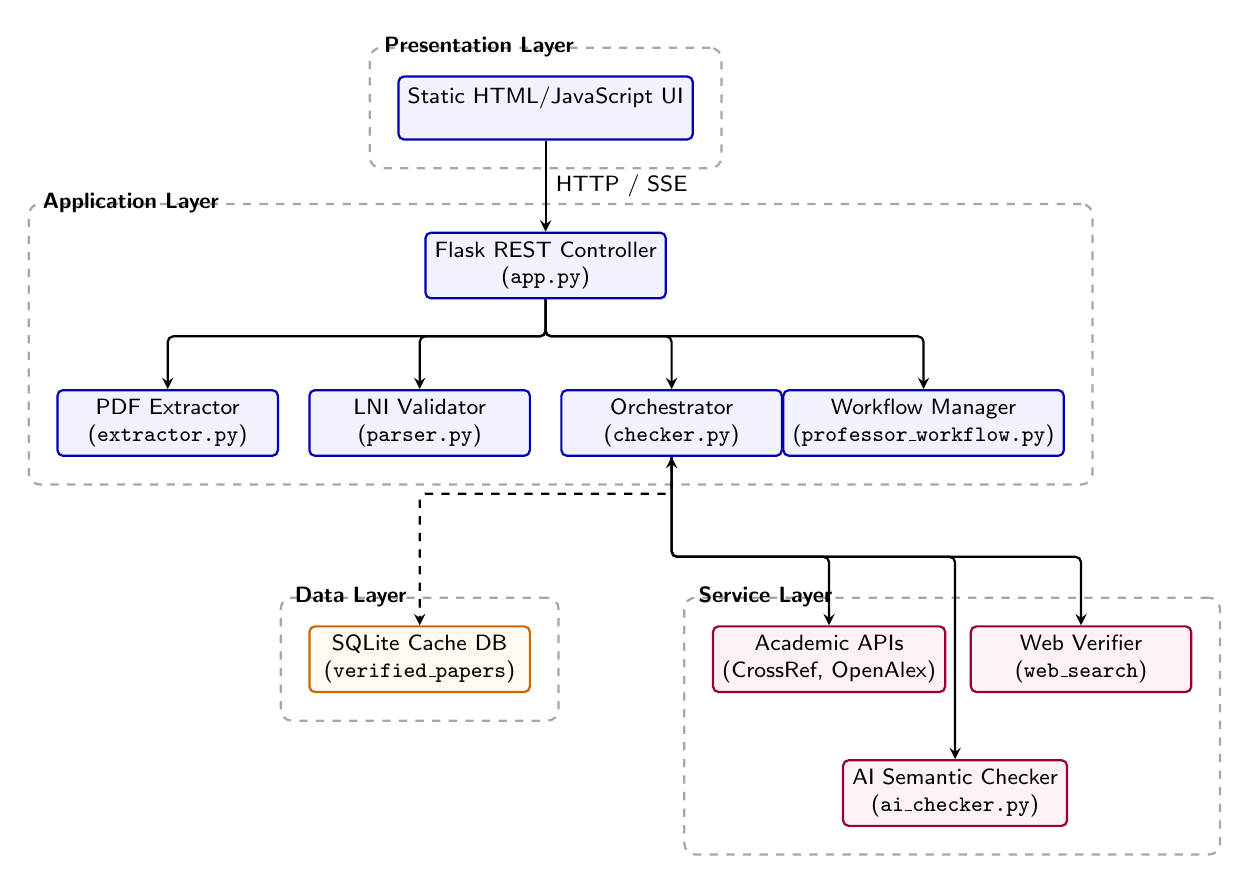
\begin{tikzpicture}[
    font=\sffamily\footnotesize,
    % Background layer styling
    layer/.style={draw=gray!70, dashed, thick, rounded corners=4pt, inner sep=0.35cm},
    % Component styling
    component/.style={draw=blue!70!black, thick, rectangle, rounded corners=2pt, fill=blue!5, minimum width=2.8cm, minimum height=0.8cm, align=center},
    db/.style={draw=orange!80!black, thick, rectangle, rounded corners=2pt, fill=orange!5, minimum width=2.8cm, minimum height=0.8cm, align=center},
    extservice/.style={draw=purple!80!black, thick, rectangle, rounded corners=2pt, fill=purple!5, minimum width=2.8cm, minimum height=0.8cm, align=center},
    % Arrow styling with rounded corners for smooth routing
    arrow/.style={->, >=stealth, thick, rounded corners=2pt},
    darrow/.style={<->, >=stealth, thick, dashed, rounded corners=2pt}
]

% ---------------------------------------------------
% 1. NODES (Positioned on a strict X,Y grid)
% ---------------------------------------------------

% Presentation Layer
\node[component] (react) at (0, 1.5) {Static HTML/JavaScript UI\\};

% Application Layer
\node[component] (flask) at (0, -0.5) {Flask REST Controller\\(\texttt{app.py})};
\node[component] (extractor) at (-4.8, -2.5) {PDF Extractor\\(\texttt{extractor.py})};
\node[component] (parser) at (-1.6, -2.5) {LNI Validator\\(\texttt{parser.py})};
\node[component] (checker) at (1.6, -2.5) {Orchestrator\\(\texttt{checker.py})};
\node[component] (workflow) at (4.8, -2.5) {Workflow Manager\\(\texttt{professor\_workflow.py})};

% Data Layer (Left Side)
\node[db] (db_papers) at (-1.6, -5.5) {SQLite Cache DB\\(\texttt{verified\_papers})};

% Service Layer (Right Side)
\node[extservice] (apis) at (3.6, -5.5) {Academic APIs\\(CrossRef, OpenAlex)};
\node[extservice] (websearch) at (6.8, -5.5) {Web Verifier\\(\texttt{web\_search})};
\node[extservice] (ai) at (5.2, -7.2) {AI Semantic Checker\\(\texttt{ai\_checker.py})};

% ---------------------------------------------------
% 2. BACKGROUND LAYERS (Drawn securely behind nodes)
% ---------------------------------------------------
\begin{scope}[on background layer]
    \node[layer, fit=(react), label={[anchor=west, xshift=2pt]north west:\textbf{Presentation Layer}}] {};
    \node[layer, fit=(flask)(extractor)(workflow), label={[anchor=west, xshift=2pt]north west:\textbf{Application Layer}}] {};
    \node[layer, fit=(db_papers), label={[anchor=west, xshift=2pt]north west:\textbf{Data Layer}}] {};
    \node[layer, fit=(apis)(websearch)(ai), label={[anchor=west, xshift=2pt]north west:\textbf{Service Layer}}] {};
\end{scope}

% ---------------------------------------------------
% 3. CONNECTIONS (Orthogonal routing to avoid overlaps)
% ---------------------------------------------------

% Presentation -> App
\draw[arrow] (react) -- node[right] {HTTP / SSE} (flask);

% Flask -> App Components (Drops down, then spreads horizontally)
\draw[arrow] (flask) -- (0, -1.4) -| (extractor);
\draw[arrow] (flask) -- (0, -1.4) -| (parser);
\draw[arrow] (flask) -- (0, -1.4) -| (checker);
\draw[arrow] (flask) -- (0, -1.4) -| (workflow);

% App -> Data Layer (Routed at specific Y-heights so lines don't cross badly)
\draw[darrow] (checker.south) -- (1.6, -3.4) -| (db_papers.north);

% App -> Service Layer
\draw[arrow] (checker.south) -- (1.6, -4.2) -| (apis.north);
\draw[arrow] (checker.south) -- (1.6, -4.2) -| (websearch.north);
\draw[arrow] (checker.south) -- (1.6, -4.2) -| (ai.north); % Drops perfectly between APIs and Websearch

\end{tikzpicture}
\caption{UML Component Diagram of the System Architecture.}
\label{fig:uml_component_architecture}
\end{figure}

\section{Presentation Layer}

The presentation layer is a single-page HTML/JavaScript interface served by Flask from the \texttt{static/} directory. It uses browser JavaScript, CSS, and Server-Sent Events (SSE); it is not a React application. The interface provides five main tabs:

The \textbf{Bibliography Tab} displays parsed bibliography entries with metadata warnings. For each entry, the system shows: citation key, authors, title, venue, year, and a completeness score. Entries with missing required fields are highlighted in orange.
\begin{figure}[ht!]
    \centering
    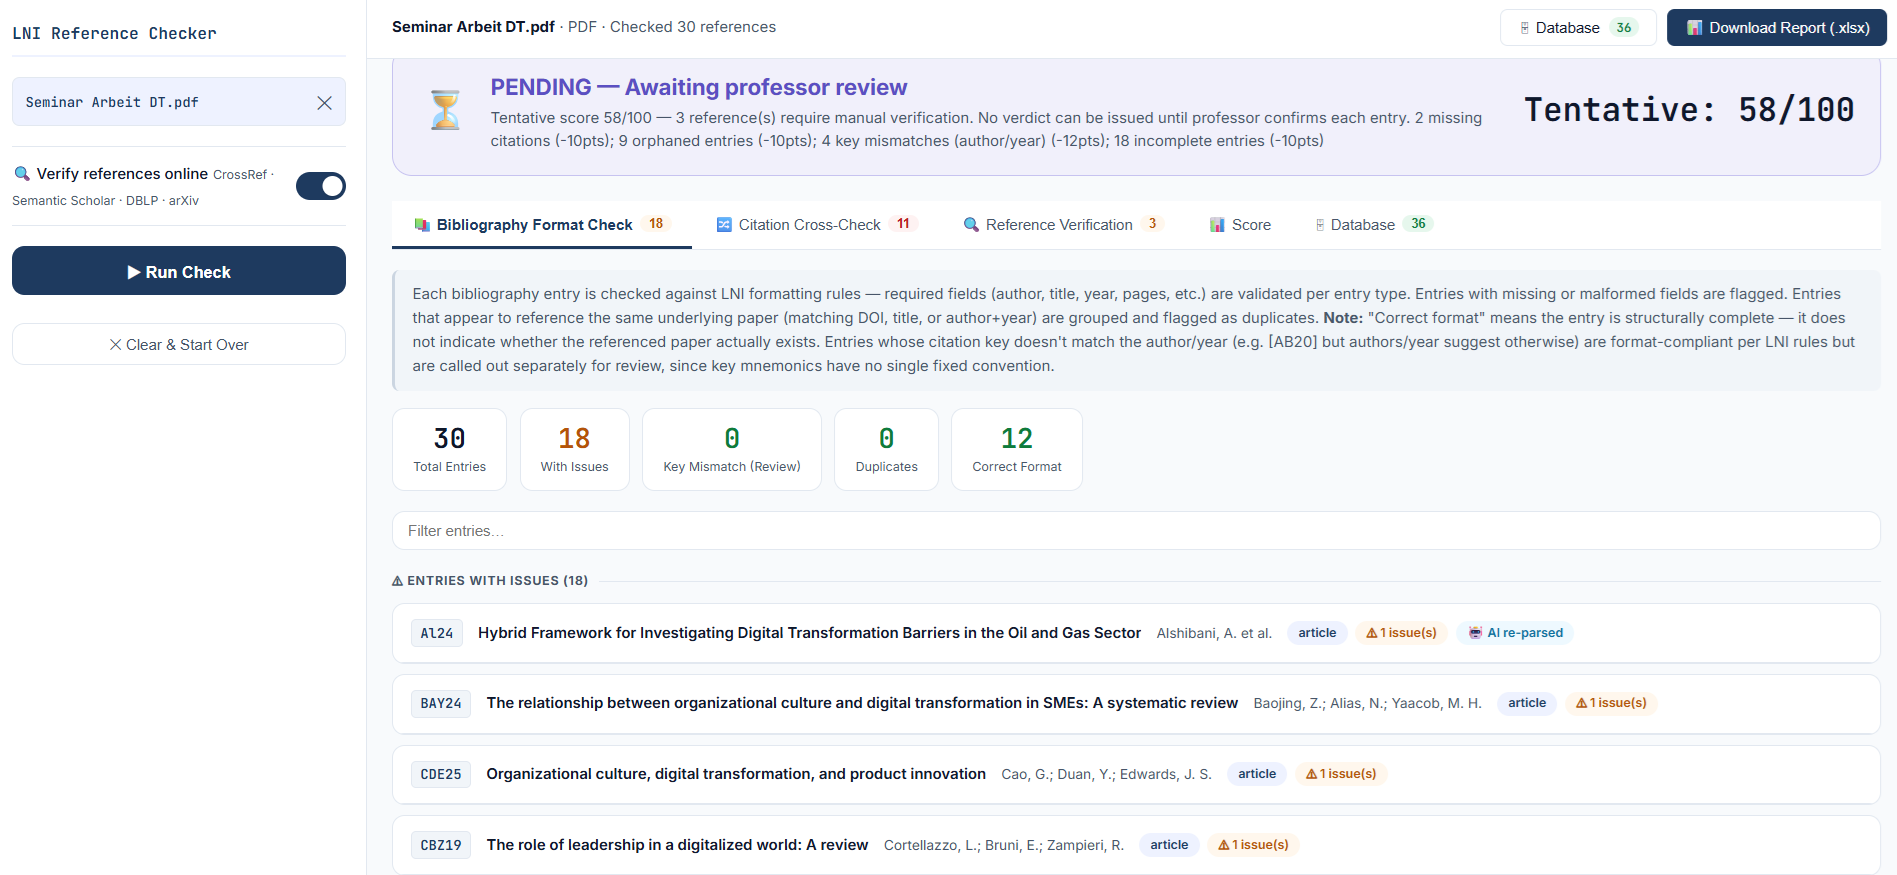
\includegraphics[width=0.8\textwidth]{figures/bib1.png}
    \caption{The Bibliography Tab displaying parsed entries with metadata completeness warnings.}
    \label{fig:Bibliography_window}
\end{figure}

\begin{figure}[ht!]
    \centering
    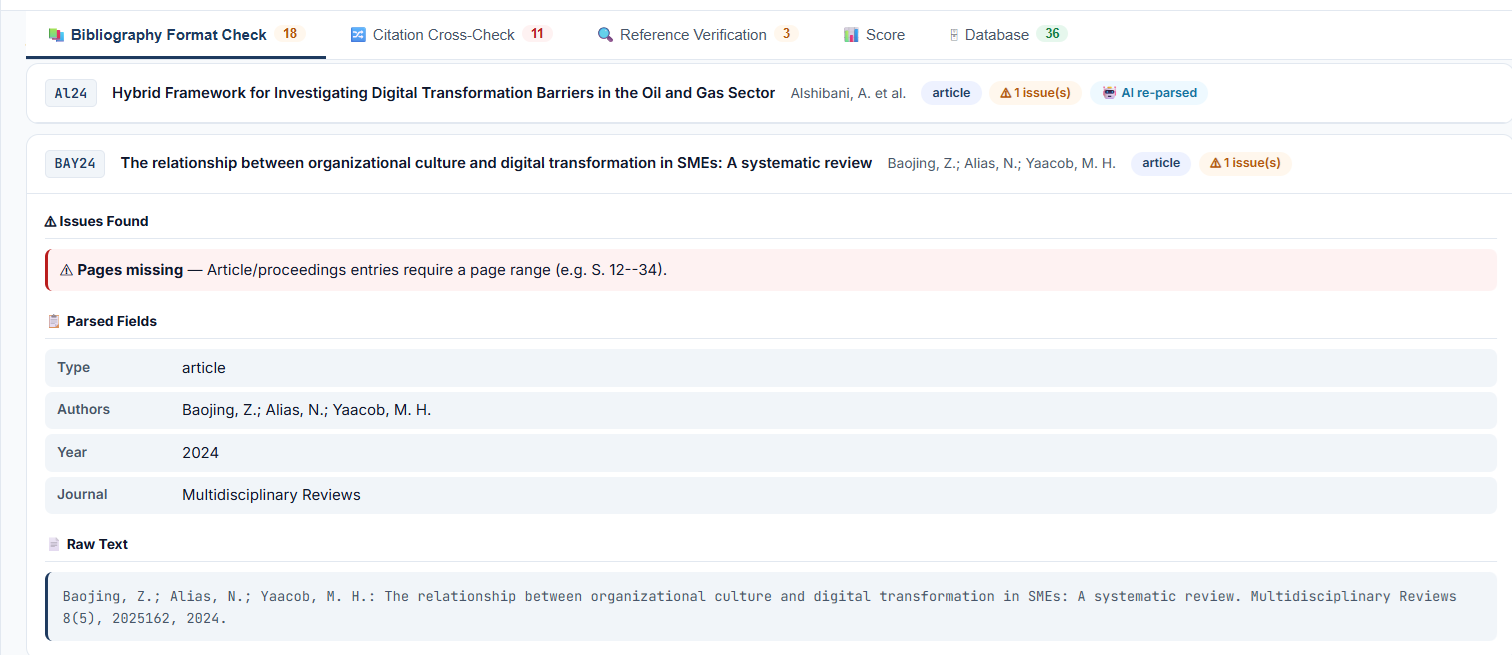
\includegraphics[width=0.8\textwidth]{figures/bib2.png}
    \caption{Detailed view of the completeness and parsed metadata for a specific entry.}
    \label{fig:Bibliography_explanation}
\end{figure}

The \textbf{Cross-Check Tab} performs citation-to-bibliography consistency analysis. It identifies missing references (cited in body text but not in bibliography), orphaned entries (in bibliography but not cited in body), and potential duplicates (very similar titles, possibly the same paper listed twice). 
\begin{figure}[H]
    \centering
    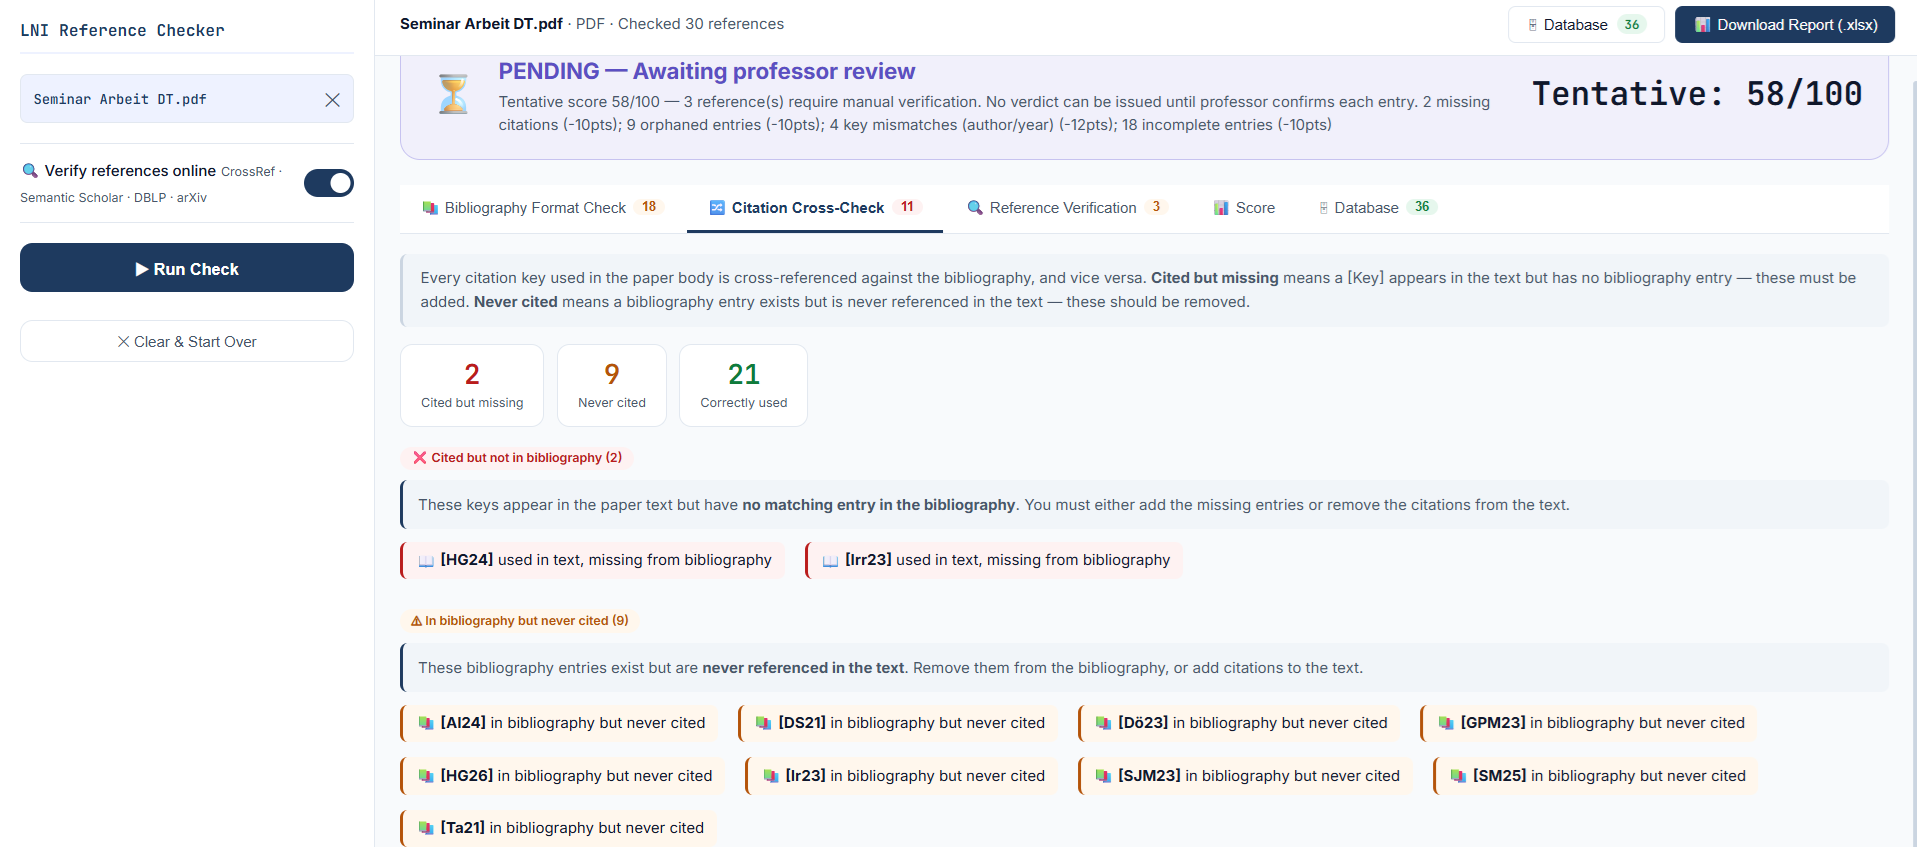
\includegraphics[width=0.8\textwidth]{figures/cross.png}
    \caption{The Cross-Check Tab identifying orphaned and missing in-text citations.}
    \label{fig:Cross-check_window}
\end{figure}

The \textbf{Verification Tab} displays verification results for each entry. For each reference, the system shows the operational result (REAL, MANUAL\_REVIEW, or another internal status), confidence score, source of verification, matched metadata, field-level mismatch warnings, and supporting evidence. A strong database candidate with an author, title, venue, or year mismatch is displayed for manual review rather than being promoted to REAL by AI. Professors use this tab to confirm legitimate references or mark confirmed fabrications.
\begin{figure}[ht!]
    \centering
    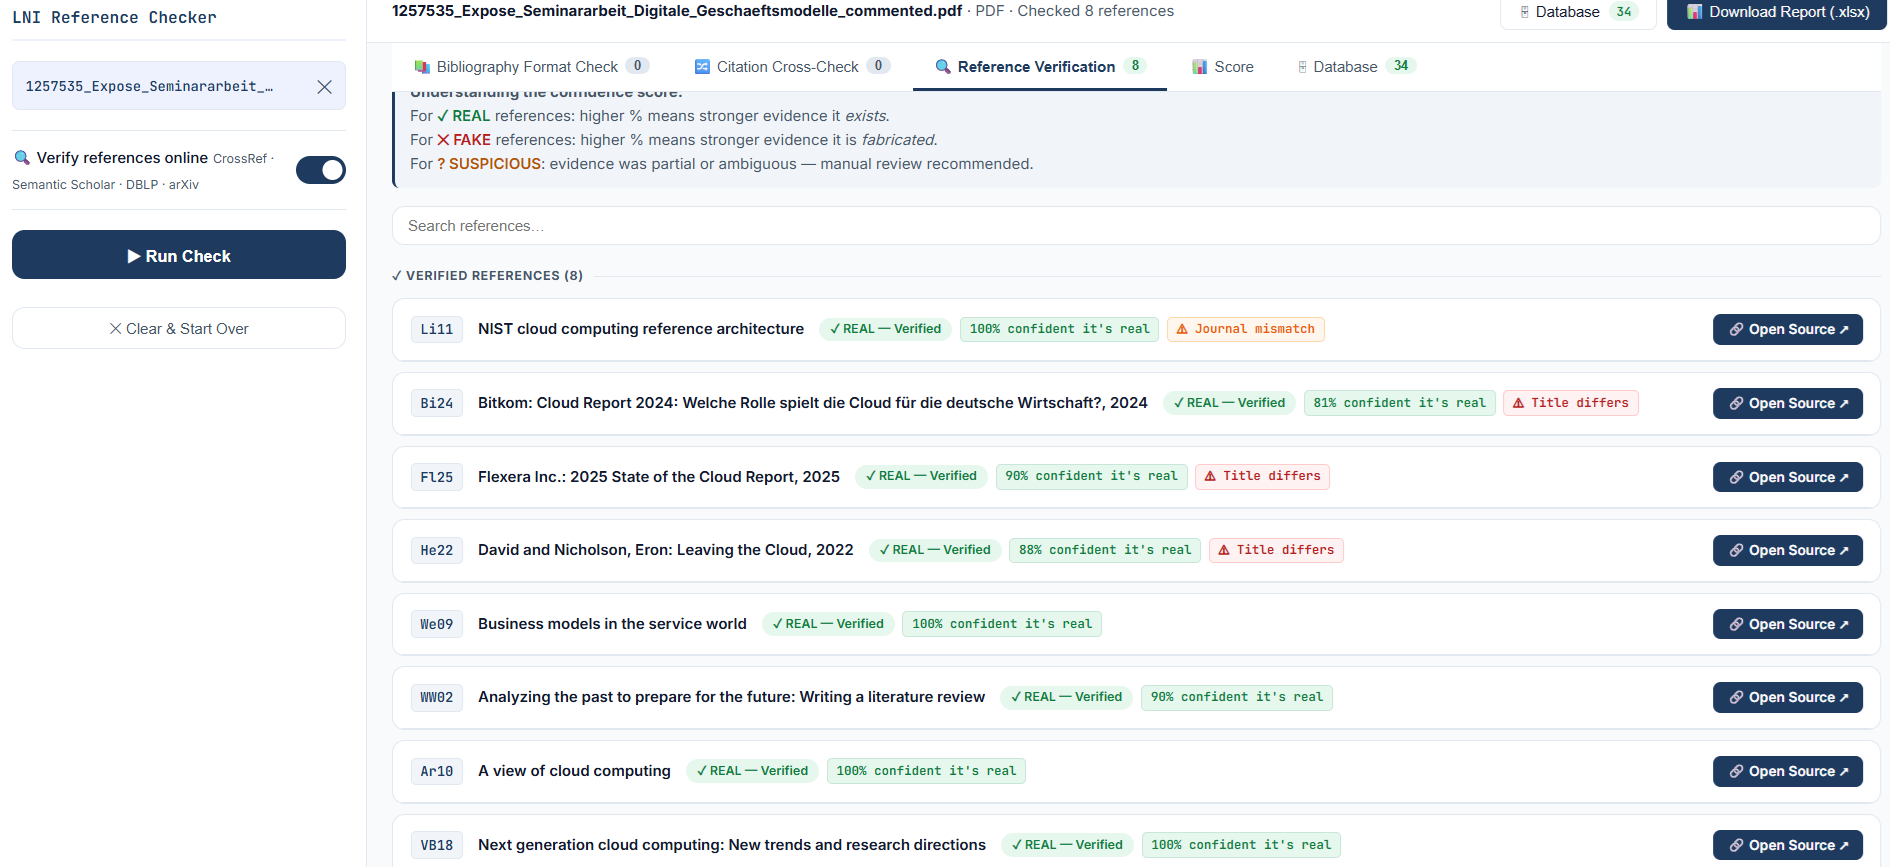
\includegraphics[width=0.8\textwidth]{figures/Results.png}
    \caption{The Verification Tab detailing verdicts, confidence scores}
    \label{fig:verification_window}
\end{figure}

The \textbf{Database Tab} allows browsing and searching the local verification cache. Users can view all previously verified papers, search by title or author, and inject new entries or correct existing ones. This tab enables manual correction of system errors and injection of papers not found by APIs.
\begin{figure}[ht!]
    \centering
    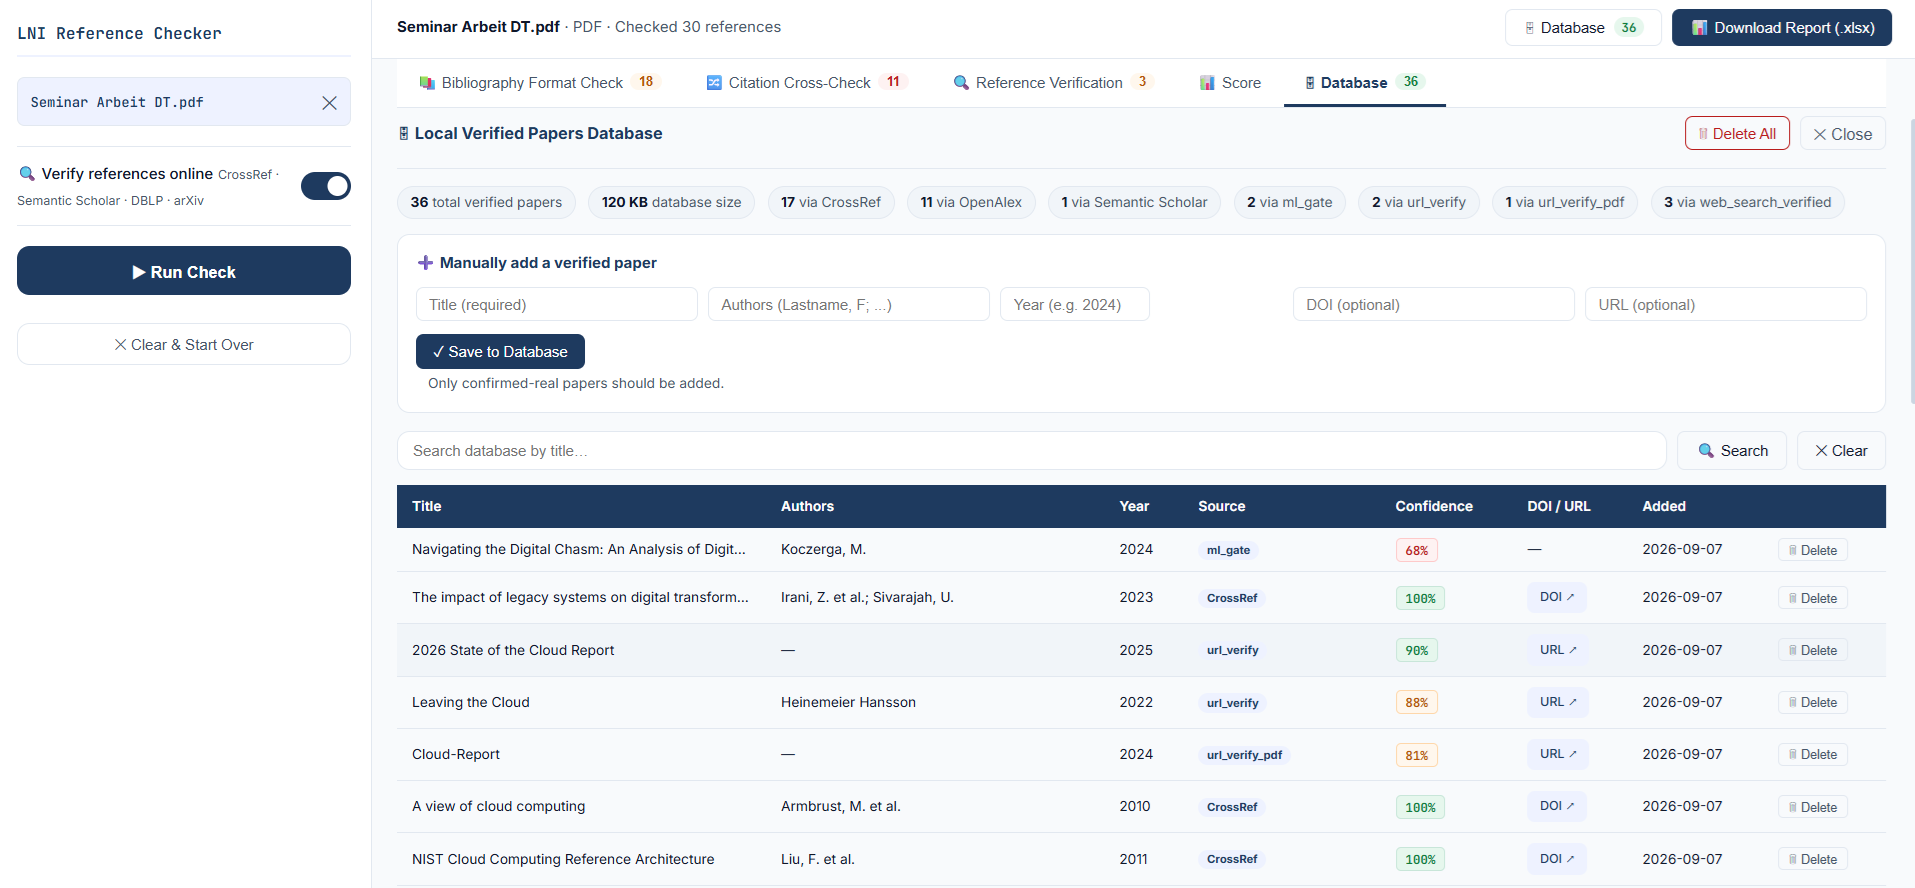
\includegraphics[width=0.8\textwidth]{figures/db.png}
    \caption{The Database Tab allowing professors to search and manually modify the local verification cache.}
    \label{fig:DB_window}
\end{figure}

The \textbf{Score Tab} provides a comprehensive overview of the evaluation metrics for the submitted document. It summarizes completeness issues, citation cross-check results, verification outcomes, manual-review items, and penalty deductions to help the professor assess the overall quality of the citations.

\begin{figure}[ht!]
    \centering
    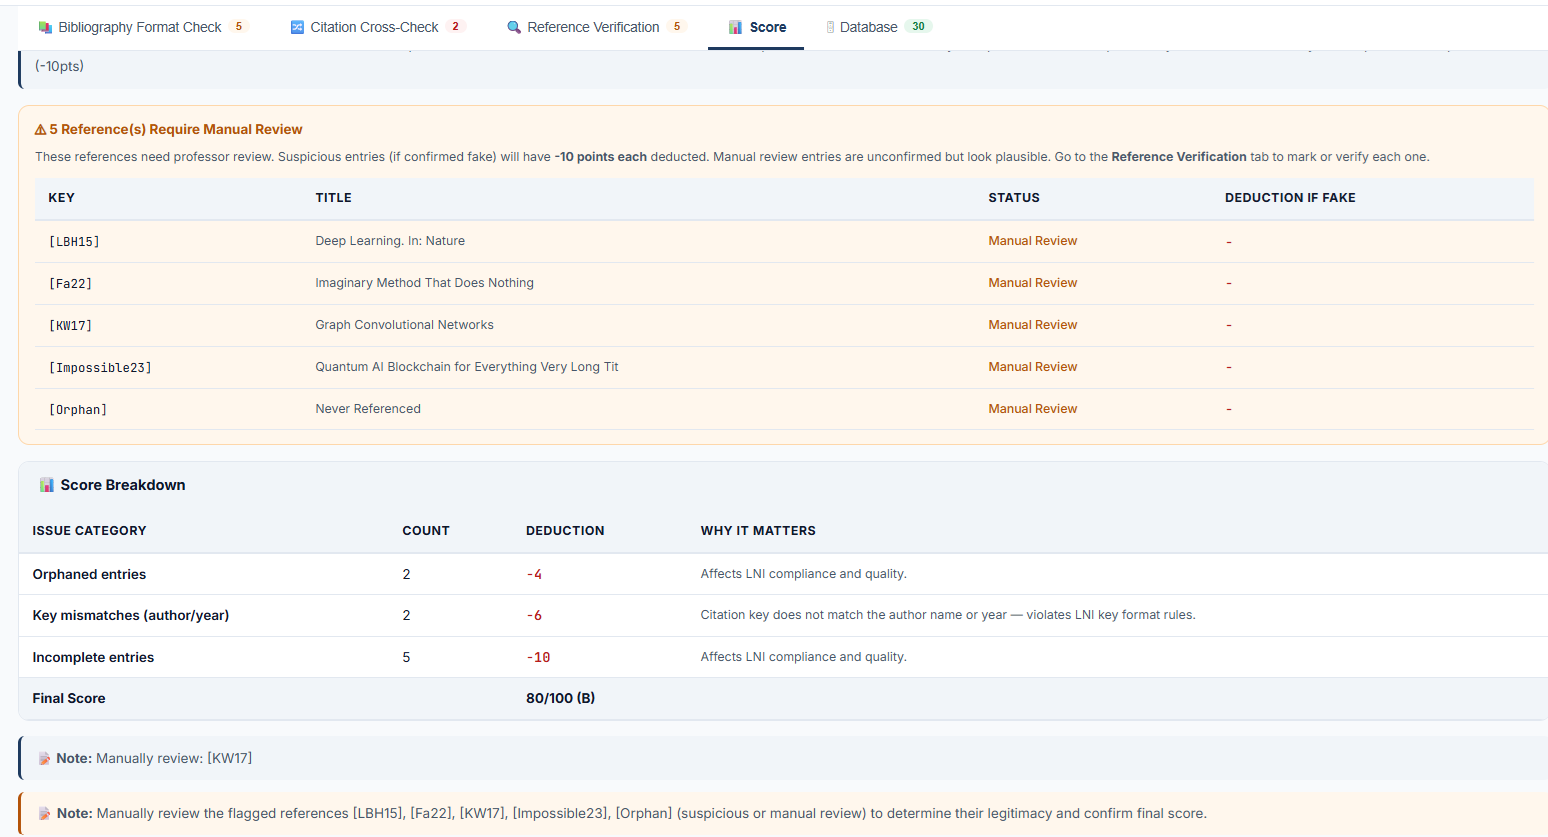
\includegraphics[width=0.85\textwidth]{figures/score_tab.png}
    \caption{The Score Tab summarizing the overall citation quality and verification metrics.}
    \label{fig:score_tab}
\end{figure}

All tabs are rendered by the browser from the JSON result assembled by Flask. During processing, Server-Sent Events stream progress, completion, and error messages so that the professor can follow the operation without manually refreshing the page.

\section{Application Layer}

The application layer implements core business logic via Python \cite{vanrossum2021} modules running on Flask \cite{grinberg2018}. The entry point is \texttt{app.py}, which exposes REST endpoints for file upload, verification orchestration, and result retrieval.

\subsection{REST Endpoints}

The principal endpoints exposed by the application layer are:

\begin{lstlisting}
GET  /                         — Serve the static interface
GET  /status                   — Return application and cache status
GET  /status/apis              — Check live academic API reachability
POST /check                    — Upload and process a document
GET  /api/db_stats              — Return local database statistics
GET  /api/db_contents           — Browse cached papers
POST /api/inject_paper          — Add a professor-confirmed paper
POST /api/db_delete             — Delete a cached paper
POST /api/db_delete_all         — Delete cached papers
\end{lstlisting}

\subsection{Core Processing Modules}

This layer houses the primary Python modules that process the document and orchestrate the workflow:

\begin{itemize}
    \item \textbf{Document Extractor (\texttt{extractor.py}):} Extracts text and bibliography sections from supported PDF, DOCX, and LaTeX inputs. Text-based PDFs are supported; scanned PDFs are detected as image-based and require OCR outside the application.
    \item \textbf{Bibliography Parser (\texttt{parser.py}):} Converts bibliography text into structured \texttt{BibEntry} objects. It prioritizes LNI-style keys and metadata, applies fallback heuristics for common layouts, and records missing or malformed fields for review.
    \item \textbf{Pipeline Orchestrator (\texttt{checker.py}):} Applies preliminary professor-decision and duplicate checks, validates structure, checks the local cache, queries academic sources with bounded concurrency, and retains partial matches for field-level review.
    \item \textbf{Workflow Manager (\texttt{professor\_workflow.py}):} Prioritizes references for review and summarizes review risks. Professor-confirmed papers are stored through the application database workflow so they can be reused in later checks.
\end{itemize}

\section{Service Layer}

The service layer encapsulates all external integrations required for verification, strictly decoupling internal logic from third-party API changes.

\begin{itemize}
    \item \textbf{Academic Database APIs:} The checker includes DOI/CrossRef lookup, OpenAlex \cite{openalex2024}, CrossRef \cite{crossref2024}, Semantic Scholar \cite{semanticscholar2024}, DBLP, arXiv \cite{arxiv2024}, PubMed, DataCite, OpenAIRE, BASE, Google Scholar, and ResearchGate source paths. Each response is converted into a common metadata record containing fields such as title, authors, year, venue, DOI, and URL when available. Source access is bounded and may be affected by rate limits or network failures.
    \item \textbf{URL Validation Service (\texttt{web\_search\_verifier.py}):} Fetches URLs to verify grey literature. It extracts page text using BeautifulSoup and implements heuristics to detect bot-blocking (Cloudflare, reCAPTCHA), gracefully falling back to web search if blocked.
    \item \textbf{Web Search Service:} Interfaces with DuckDuckGo to issue search queries using parsed titles and authors, retrieving text snippets to provide context for unverified papers.
    \item \textbf{AI Semantic Checker (\texttt{ai\_checker.py}):} Connects to the configured language-model provider and evaluates unresolved references using the parsed metadata and available source evidence. It supplies explanations and risk factors, but cannot override a deterministic title, author, venue, or year mismatch. Repeated AI requests may be served from the configured response cache.
\end{itemize}

\section{Data Layer}

The data layer is managed by \texttt{local\_db.py} and utilizes SQLite \cite{sqlite2026} to cache verified papers and professor review decisions.

\subsection{Database Schema and Optimizations}

\begin{lstlisting}[language=SQL]
CREATE TABLE verified_papers (
    id INTEGER PRIMARY KEY AUTOINCREMENT,
    title_norm TEXT UNIQUE NOT NULL,    -- dedup key
    author_norm TEXT,                   -- normalized first author
    title_blob BLOB NOT NULL,           -- zlib-compressed title
    authors_blob BLOB,                  -- zlib-compressed authors
    year INTEGER,
    doi TEXT,
    url TEXT,
    source TEXT NOT NULL DEFAULT 'unknown',
    confidence REAL NOT NULL DEFAULT 1.0,
    confirmed_real INTEGER NOT NULL DEFAULT 1,
    added_date TEXT NOT NULL,
    last_seen TEXT NOT NULL
);
\end{lstlisting}

The title and author strings are stored in zlib-compressed fields. The cache uses a normalized title key with SQLite indexes for efficient lookup, together with author, year, DOI, URL, source, confidence, and timestamp fields. Journal or venue metadata is not consistently stored in this schema, so a cache hit cannot independently validate every bibliographic field. Concurrent access is managed using SQLite's WAL (write-ahead logging) mode.

\section{Verification Pipeline in Detail}

The document-level workflow first extracts and parses the submission, applies any available parsing improvements, checks citation-to-bibliography consistency, and identifies duplicate entries. For each unique bibliography entry, the verifier then applies two preliminary control checks. First, it checks whether a professor has already recorded a decision. This is a manual override, not an external evidence source. Second, it checks whether the entry is a duplicate of another bibliography entry; duplicates inherit the canonical entry's result.

After these control checks, the evidence-based verification pipeline proceeds in the following order:

\begin{enumerate}
    \item Structural metadata validation
    \item Local SQLite cache lookup
    \item Academic source queries
    \item URL and web evidence, where available
    \item AI-assisted assessment of unresolved cases
    \item Deterministic final verdict and manual-review routing
\end{enumerate}

The local cache is therefore the first evidence-based verification source. External services are used only when the cache does not provide a valid metadata match. A strong candidate with a title, author, venue, or year mismatch is retained as a partial match and routed to manual review rather than being discarded or promoted to REAL.

\begin{figure}[ht!]
\centering
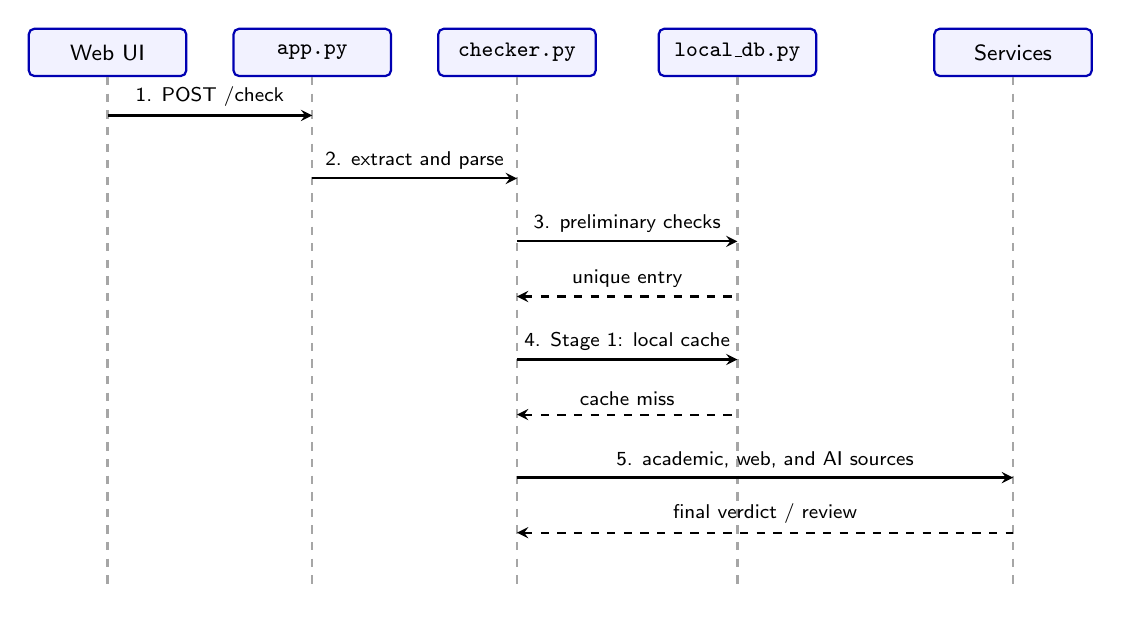
\begin{tikzpicture}[
    font=\sffamily\footnotesize,
    lifeline/.style={draw=gray!70, dashed, thick},
    entity/.style={draw=blue!70!black, fill=blue!5, thick, rounded corners=2pt, minimum width=2cm, minimum height=0.6cm, align=center},
    msg/.style={->, >=stealth, thick},
    ret/.style={<-, >=stealth, dashed, thick}
]

% 1. Entities (X-coordinates compressed)
\node[entity] (ui) at (0,0) {Web UI};
\node[entity] (app) at (2.6,0) {\texttt{app.py}};
\node[entity] (chk) at (5.2,0) {\texttt{checker.py}};
\node[entity] (db) at (8.0,0) {\texttt{local\_db.py}};
\node[entity] (ext) at (11.5,0) {Services};

% 2. Lifelines
\draw[lifeline] (ui.south) -- (0, -6.8);
\draw[lifeline] (app.south) -- (2.6, -6.8);
\draw[lifeline] (chk.south) -- (5.2, -6.8);
\draw[lifeline] (db.south) -- (8.0, -6.8);
\draw[lifeline] (ext.south) -- (11.5, -6.8);

% 3. Messages
\draw[msg] (0, -0.8) -- node[above, scale=0.9] {1. POST /check} (2.6, -0.8);

\draw[msg] (2.6, -1.6) -- node[above, scale=0.9] {2. extract and parse} (5.2, -1.6);

\draw[msg] (5.2, -2.4) -- node[above, scale=0.9] {3. preliminary checks} (8.0, -2.4);
\draw[ret] (5.2, -3.1) -- node[above, scale=0.9] {unique entry} (8.0, -3.1);

\draw[msg] (5.2, -3.9) -- node[above, scale=0.9] {4. Stage 1: local cache} (8.0, -3.9);
\draw[ret] (5.2, -4.6) -- node[above, scale=0.9] {cache miss} (8.0, -4.6);

\draw[msg] (5.2, -5.4) -- node[above, scale=0.9] {5. academic, web, and AI sources} (11.5, -5.4);
\draw[ret] (5.2, -6.1) -- node[above, scale=0.9] {final verdict / review} (11.5, -6.1);

\end{tikzpicture}
\caption{Sequence Diagram of the verification pipeline.}
\label{fig:uml_pipeline_sequence}
\end{figure}

\subsection{Stage 1: Local Cache Lookup}

After professor-decision, duplicate, and structural checks, the system queries the local SQLite database for previously verified papers. The lookup uses a normalized title key and then checks the cited authors against the cached authors. A cached record is accepted only when the relevant metadata checks pass. The cache currently stores title, authors, year, DOI, URL, source, confidence, and timestamps; journal or venue metadata is not consistently stored.

\textbf{Rationale:} Papers often appear in multiple submissions or are verified multiple times. A valid cache hit avoids external API requests and reduces repeated work. A cache miss, or a cached record rejected because of an author mismatch, continues to the academic-source stage.

\subsection{Stage 2: Academic Source Queries}

For references not confirmed by the cache, the system uses a bounded source chain containing DOI/CrossRef lookup, arXiv identifier lookup, OpenAlex, CrossRef, Semantic Scholar, DBLP, arXiv search, PubMed, DataCite, OpenAIRE, BASE, Google Scholar, and ResearchGate paths. The source functions run with bounded concurrency and per-source rate and timeout controls. The verifier returns early when a trusted complete match is found, but it also retains the strongest partial candidate when the title is close and other metadata fields differ.

For each candidate, the system compares the title, authors, year, venue, and DOI when those fields are available. The title similarity configuration uses a default threshold of 0.80, while author comparison uses source-aware overlap rules. Publication years must match exactly when both years are comparable. A candidate with any substantive title, author, venue, or year mismatch is not promoted to REAL; it is returned as a partial match and routed to manual review with the mismatched fields displayed.

\subsection{Stage 3: URL and Web Evidence}

For references that contain URLs but lack a conclusive academic-source match, the system can fetch and inspect the referenced page. The web verifier extracts visible page text, compares it with the cited title, and detects common bot-blocking responses. URL evidence can support verification of grey literature, technical reports, white papers, and institutional material, but an HTTP success response alone does not prove that the cited publication is correct. Weak or ambiguous URL evidence continues to the next stage rather than automatically producing REAL.

\subsection{Stage 4: AI-Assisted Assessment}

For references that remain unresolved after the cache, academic sources, and available web evidence, the application sends the parsed metadata and available source results to the configured AI verifier. Web-search evidence may be included when available. The AI produces a confidence assessment, explanation, and risk factors for the professor.

\begin{quote}
"Given the citation metadata and available source evidence, assess whether the reference is supported and explain any uncertainty."
\end{quote}

AI output is advisory. It cannot override a deterministic metadata mismatch. If a likely paper was found but the cited author, title, venue, or year differs, the final result remains MANUAL\_REVIEW even when the AI considers the paper likely real. The system also never independently assigns the final FAKE verdict; that decision belongs to the professor.



\section{Professor Workflow Manager (\texttt{professor\_workflow.py})}

The workflow manager provides prioritization, manual-review support, and database-management capabilities for professors. It serves as the bridge between automated evidence collection and the human decision that resolves ambiguous references.

\subsection{Manual Verdict Marking}

Professors can review references marked as MANUAL\_REVIEW or SUSPICIOUS and then record a final decision based on the displayed source evidence and corrected metadata:

\textbf{Confirm as REAL:} When a professor independently verifies a reference that the system could not confirm automatically, they can save the paper as confirmed real. The application stores its available title, authors, year, DOI, and URL in the SQLite cache with high confidence, allowing future submissions to benefit from the decision.

\textbf{Mark as FAKE:} When a professor confirms that a reference does not exist or is materially fabricated, they can mark it as FAKE. The system never unilaterally assigns this final verdict; this judgment is reserved exclusively for professors to minimize false accusations.

\subsection{Manual Database Injection}

Professors can inject verified papers directly into the SQLite cache through the Database Tab. This addresses scenarios where automated verification fails to find legitimate references, such as German conference proceedings not indexed by CrossRef, grey literature lacking DOIs, recent publications not yet in databases, or system parsing errors.



% ============================================================================
\chapter{Scientific Methodology}
% ============================================================================

Having established the system's structural architecture and overall verification pipeline, the scientific foundation of the LNI Reference Checker rests upon a systematic approach to extracting, parsing, and verifying bibliographic information. This chapter explains how the implementation processes supported documents, compares metadata with external records, reports field-level mismatches, and routes unresolved cases to professor review. The system is designed to identify suspicious or inconsistent references; it does not independently assign the final FAKE verdict.

\section{Document Processing and Bibliography Extraction}

PDF documents present a notoriously complex landscape for automated text extraction. Because the format was originally engineered for visual fidelity and printing rather than semantic data accessibility, recovering a perfectly structured bibliography requires multi-layered processing heuristics.

\subsection{Layout-Aware Text Extraction and Normalization}

\textbf{Rationale and Execution:} The extraction process uses \texttt{pdfplumber} \cite{singer2016} and a simpler \texttt{pypdf} fallback for PDF text recovery. Layout-aware extraction and cleanup heuristics are used to separate document body text from the bibliography, repair URLs and line-break artifacts, and remove common page-header and page-number noise. Text-based PDFs are the primary supported PDF input; scanned or image-only PDFs are detected as scanned and require OCR outside the application.

\textbf{Handling Ligatures and Diacritics:} A significant methodological challenge involves the programmatic handling of typographic ligatures. Ligatures are combined glyphs used in professional typesetting to represent multiple character sequences as a single printed unit. Common examples include explicit combinations such as \ae{} and \oe{}, or the visual fusion of ``f'' and ``i''. When extracted from a PDF text layer, these single-glyph combinations frequently decode as missing characters or corrupted Unicode symbols, which inherently fail exact-string database lookups. 

To mitigate this, the system preserves Unicode text where possible and applies targeted normalization during metadata comparison. Titles and metadata are normalized for HTML entities, whitespace, case, punctuation, selected diacritics, simple LaTeX-brace expressions, and selected stop words. Author surnames receive additional normalization for diacritics, punctuation, name particles, and limited prefix similarity. This improves matching against records that use different typographic representations without replacing the original displayed citation.

\textbf{Artifact Removal and Hyphenation:} Extracted PDF text may contain page numbers, repeated headings, and line-break artifacts. The extractor applies document-specific cleanup rules, collapses unsuitable blank lines, repairs URLs and common hyphen/space artifacts, and limits the bibliography using recognized section boundaries. These heuristics improve extraction but cannot guarantee perfect recovery from badly encoded or image-only PDFs; incomplete results are therefore surfaced for review.

\textbf{Encoding and File Handling:} The extractor works with the text returned by the PDF, DOCX, or LaTeX parsing libraries and applies Unicode normalization where needed. Uploaded documents are held temporarily during processing and removed after the request. The implementation does not claim universal recovery of legacy encodings; unreadable or scanned inputs are reported as incomplete rather than silently treated as verified text.

\subsection{Bibliography Format Detection and Parsing}

Academic documents may contain LNI entries mixed with other layouts. The parser is primarily designed for LNI-style keys and bibliography structure, with fallback heuristics for common author--title--venue, book, proceedings, website, and malformed arrangements.

\textbf{Format Handling:} The parser identifies bracketed citation keys and uses structural patterns such as colons, semicolons, publication years, venue markers, URLs, volume information, and page ranges. It recognizes numeric and LNI-style keys and reports malformed or uncertain entries. It should not be interpreted as a complete independent parser for every citation standard.

\textbf{LNI Extraction and Fallback Parsing:} For LNI-style entries, the parser extracts the bracketed key, identifies the author--title boundary, extracts title, year, pages, venue, publisher, DOI, and URL fields, and infers an entry type. Semicolon-separated \texttt{Lastname, Firstname} authors are preferred, but common variations are tolerated. Missing or malformed fields are retained as completeness issues.

For uncertain entries, the application may use the configured AI parsing step to suggest missing metadata fields. This is an assistance mechanism, not a replacement for deterministic parsing: AI suggestions are applied cautiously and the resulting entry remains subject to completeness checks and external verification.

\textbf{Completeness Evaluation:} Extraction is followed by required-field validation based on the inferred entry type. For example, article and proceedings entries are expected to contain authors, title, venue/booktitle, year, and pages, while books require authors, title, publisher, and year. Missing or malformed fields generate explicit completeness issues and can send the entry to manual review. The system does not use a universal completeness score threshold of 0.7 as the sole decision rule.

\section{Similarity Metrics and Metadata Matching}

Following extraction and parsing, the verification pipeline relies on robust, algorithmically driven similarity metrics to match citations found in documents against official entries recovered from external academic databases. As introduced conceptually in Chapter 2, these metrics are physically implemented in the backend to explicitly balance precision against recall.

\subsection{Title Similarity Computation}

\textbf{Rationale and Execution:} Traditional exact-string matching is entirely unsuited for academic reference verification because manual citations frequently suffer from typographical errors, OCR artifacts, and omitted subtitles. A robust system requires approximate string matching to forgive these surface-level deviations while definitively rejecting entirely different papers.

As defined in Chapter 2, the system calculates a proportionate match score by combining two distinct text-comparison algorithms. First, it utilizes the \texttt{rapidfuzz} library \cite{bachmann2024} to compute a token-sorted Levenshtein edit distance. Token sorting is critical: it splits the string into individual words, reorganizes them into alphabetical order, and then computes the distance. This makes the metric immune to word-order swaps (e.g., easily matching ``Deep Learning for Natural Language'' to ``Natural Language Processing with Deep Learning''). Second, the system calculates a Word Overlap metric by counting shared significant words (defined as tokens containing five or more characters). 

Before computation, both titles are aggressively normalized (lowercased, diacritics removed, spaces collapsed, and English stopwords stripped). The final similarity score is computed as:

\begin{equation}
\text{Sim}_{\text{title}} = 0.75 \cdot \text{FuzzyRatio}(t_1, t_2) + 0.25 \cdot \text{WordOverlap}(t_1, t_2)
\end{equation}

This formula is heavily utilized during the API verification phase. The 0.75 weight deliberately prioritizes exact character-level spelling matches to catch OCR typos, while the 0.25 weight acts as a semantic safety net for titles where entire words have been heavily transposed or abbreviated.

\subsection{Author Overlap Measurement}

\textbf{Rationale and Execution:} Academic author lists are highly variable. Students routinely truncate long author lists using ``et al.,'' omit middle initials, or swap first and last names. Relying on exact author-string matching would result in a massive false-positive rejection rate.

As outlined in Chapter 2, the system extracts and normalizes surnames from the parsed citation and the source record. It counts how many cited surnames can be matched and divides by the smaller of the cited and source author-list sizes. This supports abbreviated citations while still detecting a complete author mismatch:

\begin{equation}
\text{Overlap}_{\text{author}} = \frac{\text{matched cited surnames}}{\min(\text{cited author count},\text{source author count})}
\end{equation}

Because this denominator is based on the smaller list, a citation using ``et al.'' is not automatically penalized when the source record contains additional authors. Any substantive author mismatch is nevertheless reported explicitly and routes the reference to manual review.

\section{Confidence Scoring and Multi-Source Aggregation}

Because references traverse different paths depending on their accessibility (cache, APIs, URLs, web evidence, and AI), the system records source-specific confidence values in the range 0.0--1.0. These values describe the strength of available evidence, while deterministic field checks control whether a reference can be presented as REAL or must be routed to MANUAL\_REVIEW.

\subsection{Method-Specific Computations and Thresholds}

The system combines configurable similarity thresholds with required-field checks. Thresholds help identify candidate records, but a high similarity score alone does not prove that all cited metadata is correct.
\begin{itemize}
    \item \textbf{Local Cache Lookup:} The cache uses a normalized title key and checks author overlap before accepting a record. A cache hit is accepted only when the relevant metadata checks pass; there is no universal 0.95 title-similarity rule at lookup time, and venue metadata is not consistently stored in the cache.
    \item \textbf{Academic Sources:} The default title-candidate threshold is 0.80 and author comparison uses source-aware surname overlap. When both years are comparable, they must match exactly. Candidate records are compared field by field. A title wording, author, venue, or year mismatch is retained as evidence but forces MANUAL\_REVIEW rather than being converted into REAL by an AI confidence score.
\item \textbf{URL Validation:} This is invoked for references that contain URLs but lack conclusive matches from academic APIs. Its purpose is to verify the existence of grey literature, such as technical reports, white papers, and preprints, that is frequently not indexed by traditional academic databases. The verification is performed by fetching the URL provided in the bibliography entry and analysing the retrieved page content.

The verification process proceeds as follows. First, the system extracts the URL from the bibliography entry. Second, it downloads the HTML content of the page using the BeautifulSoup library. Third, it extracts the visible text from the HTML, stripping out code, styling, and navigation elements. Fourth, it searches for significant keywords from the cited title within the extracted text. Significant keywords are defined as words of five or more characters, excluding common English stop words such as ``the'', ``and'', and ``for''. Fifth, it assigns a confidence score based on the number of keywords found.

The web verifier treats HTTP success and title evidence as supporting signals, not as an automatic REAL decision. A page may be related, incomplete, blocked, or unrelated even when it returns HTTP 200. The resulting evidence is passed to the final decision process together with the parsed metadata and any academic-source results.

A weak web result does not terminate processing. The reference can proceed to AI-assisted assessment, but unresolved or inconsistent metadata remains MANUAL\_REVIEW.

The following example illustrates the process. Consider a bibliography entry citing the paper ``Attention Is All You Need'' by Vaswani et al., published in 2017, with the URL \url{https://arxiv.org/abs/1706.03762}. The system extracts the URL and inspects the visible page text for significant title keywords. If the page supports the cited title and authors, it strengthens the evidence; the reference is still checked against the remaining metadata and is routed to manual review if a substantive mismatch remains.

\item \textbf{AI-Assisted Assessment:} This is used for unresolved references after cache, academic-source, and available web evidence checks. It relies on semantic reasoning over the citation metadata and available evidence, but remains advisory.

The application sends the unresolved citation metadata and available source evidence to the configured language model. The model returns a structured assessment containing a verdict suggestion, confidence, explanation, and risk factors when the provider responds successfully. The result is used to explain uncertainty and prioritize review; it is not treated as independent proof of publication existence.

The AI confidence reflects the model's assessment, not a deterministic database match. A high value may indicate strong supporting context, while a moderate or low value indicates uncertainty. Most importantly, AI cannot override a deterministic title, author, venue, or year mismatch, and the application never uses AI alone to assign the final FAKE verdict.

The following example illustrates the process. Consider again the bibliography entry citing ``Attention Is All You Need'' by Vaswani et al. from 2017. If the available evidence supports the title and author list, the AI may provide a strong explanation that the paper is likely real. If the cited year or authors differ from the source record, the deterministic mismatch rule takes precedence and the result remains MANUAL\_REVIEW.

The resulting confidence is reported alongside the source evidence. The application does not apply one universal adaptive weighted-average formula across cache, APIs, URL evidence, and AI; the final operational status is determined by trusted evidence and deterministic field checks.
\end{itemize}

\subsection{Evidence Precedence Across Verification Paths}
The implementation does not combine every available signal through one universal adaptive-weighting equation. Instead, it applies an evidence hierarchy and deterministic field checks. Previously recorded professor decisions have the highest operational priority, followed by valid local-cache matches and complete academic-source matches. URL and AI evidence support unresolved cases but cannot override a substantive title, author, venue, or year mismatch.

This precedence is reflected directly in the backend logic: the verifier checks professor review decisions first, then duplicate status, then structural validation, then the local SQLite cache, and only then continues to academic database queries. URL and web evidence are used as supporting checks for unresolved or grey-literature references, while AI output is advisory and explanatory. The final verdict therefore follows the strongest reliable evidence available, not a universal weighted average across all sources.

In practice, a cache hit is accepted only when the normalized title and author checks pass; a candidate academic record is accepted only when the relevant title, author, venue, and year checks are sufficiently consistent; and a URL is treated as supporting evidence rather than direct proof. AI confidence values are reported for prioritization and explanation, but they cannot override a deterministic title, author, venue, or year mismatch. This is the design used by the actual implementation in \texttt{checker.py}, where the system returns MANUAL\_REVIEW when required metadata is inconsistent and never assigns FAKE without professor review.

The practical consequence is that the system's confidence display is best understood as source-specific evidence strength rather than as a mathematically combined score across every stage. A high-confidence cache hit or a strong academic match can lead to REAL, while a partial or conflicting match remains MANUAL\_REVIEW even if the AI explanation is favorable. This distinction is essential for faithful interpretation of the verification workflow and matches the operational checks used in the code.

The following table summarises the evidence-precedence order and explains the rationale for each operational treatment.

\begin{table}[H]
\centering
\begin{tabular}{
    >{\raggedright\arraybackslash}p{0.28\textwidth}
    >{\raggedright\arraybackslash}p{0.60\textwidth}
}
\toprule
\textbf{Evidence path} & \textbf{Operational treatment} \\
\midrule
Professor decision & Highest-priority manual override; reused for the same reference. \\
Local cache & Accepted only after normalized-title and author checks pass. \\
Academic source & Strongest external evidence; all available metadata fields are compared. \\
URL/web evidence & Supporting evidence for grey literature and unresolved records. \\
AI assessment & Explanatory and advisory; cannot override deterministic mismatches. \\
\bottomrule
\end{tabular}
\caption{Evidence precedence used by the implemented verification pipeline.}
\label{tab:evidence_precedence}
\end{table}

The implementation therefore reports confidence as supporting context rather than as a universal mathematical combination of all stages. A complete trusted match may be displayed as REAL, while a partial match, missing field, or substantive metadata mismatch is displayed as MANUAL\_REVIEW regardless of the AI confidence value.



\section{Grey Literature and Non-Traditional Publication Handling}

Academic verification databases globally prioritize peer-reviewed journal articles and established conference proceedings. Technical reports, white papers, industry publications, and preprints receive minimal or delayed indexing. The system must actively adapt its verification scoring methodology to handle these grey literature types to prevent unfairly penalizing students.

\subsection{Grey-Literature Handling}
Industry reports, white papers, technical reports, and preprints may be absent from one or more academic databases. The checker therefore uses URLs, web evidence, and alternative source paths where available. These sources improve recall but do not automatically relax the deterministic requirement that a substantive title, author, venue, or year mismatch be shown for manual review.

\subsection{German Academic Whitelist}
Furthermore, because global APIs like CrossRef frequently lack coverage for regional European conferences, the system implements a domain-specific Whitelist mechanism tailored to the German academic landscape. The system is pre-populated with a trust-tier database of known Gesellschaft für Informatik (GI) venues. 

\begin{lstlisting}[language=Python, caption={Pre-populated whitelist categorizing German venues by trust level.}]
def _init_default_whitelist():
    german_venues = [
        # === GI / LNI series (high trust) ===
        ("Lecture Notes in Informatics (LNI)", "series", "Germany", "high"),
        ("LNI", "series", "Germany", "high"),
        ("GI Jahrestagung", "conference", "Germany", "high"),
        ("INFORMATIK", "conference", "Germany", "high"),
        ("Gesellschaft fur Informatik", "organization", "Germany", "high"),
        ("Gesellschaft für Informatik", "organization", "Germany", "high"),

        # === German DB / IS conferences ===
        ("BTW", "conference", "Germany", "high"),
        # ...
\end{lstlisting}

References targeting these specific, high-trust venues completely bypass standard global API failure penalties, effectively preventing legitimate regional publications from triggering false positive ``SUSPICIOUS'' flags simply due to a lack of international indexing.

\section{Confidence Tiers and Verdict Routing}

The source-specific confidence values described above guide presentation and review priority; they are not combined by one universal weighted-sum formula. The final operational result is determined by the evidence source and by deterministic metadata checks. This distinction is important for professors: a high confidence that a paper exists does not mean that the student's authors, title, venue, and year are all correct.

\begin{equation}
C = \text{source-specific supporting confidence}
\end{equation}

The displayed confidence is interpreted together with the source list, field checks, and mismatch explanations. It is not a substitute for those details.

Only evidence that was actually gathered is displayed. If the local cache or an academic source confirms all required fields, the result can be REAL. If a source returns a likely paper but any substantive required field differs, the result is MANUAL\_REVIEW. AI explanations can clarify the reason but cannot override this rule.

For example, an academic record may strongly support that a paper exists while showing a different publication year from the citation. The existence evidence can receive a high confidence value, but the final reference result is still MANUAL\_REVIEW with a year-mismatch explanation.

Confidence tiers guide review priority, but they do not replace the field-level verdict rules defined in Chapter 2. REAL requires a trusted complete match. MANUAL\_REVIEW covers missing, inconsistent, partial, or unresolved metadata. FAKE remains a professor-only final decision.

One point deserves emphasis. The system never assigns the final FAKE verdict. FAKE is reserved exclusively for professors, who review the evidence and decide whether a reference is fabricated. Low confidence and source exhaustion are recommendations for review, not proof of fabrication.

The system may show risk factors such as missing metadata, no database record, or inconsistent fields, but these factors are presented as evidence for human review rather than an automatic fake score.

\begin{table}[H]
\centering
\begin{tabular}{
    >{\raggedright\arraybackslash}p{0.24\textwidth}
    >{\raggedright\arraybackslash}p{0.62\textwidth}
}
\toprule
\textbf{Operational result} & \textbf{Interpretation and professor action} \\
\midrule
REAL & A trusted source confirms the reference and the required cited metadata matches. No automatic professor action is required. \\
MANUAL\_REVIEW & The paper may exist, but a required field is missing, mismatched, ambiguous, or not confirmed. Review the displayed source and mismatch details. \\
PARTIAL\_MATCH & Internal status indicating that a likely source candidate was found but metadata differs. The interface presents this as MANUAL\_REVIEW. \\
FAKE & A final professor-only decision after reviewing the available evidence. The system does not assign it independently. \\
\bottomrule
\end{tabular}
\caption{Operational results and their required human interpretation.}
\label{tab:confidence_tiers}
\end{table}




\section{Fabrication Detection and Metadata Consistency}

After the system compares a citation with available source records, it presents field-level consistency findings. These findings help identify transcription errors, wrong versions, incomplete entries, and possible fabrication, but they do not constitute an automatic FAKE decision.

\subsection{Mismatch Accumulation}
When an academic source returns a partial match, the system compares title, authors, year, venue, and DOI when those fields are available. Publication years must match exactly when both are comparable. A substantive title, author, venue, or year mismatch is explicitly labeled and routes the entry to MANUAL\_REVIEW. The number of mismatches helps the professor prioritize attention, but there is no rule that automatically converts a mismatch count into FAKE.

\subsection{LNI Key Consistency Logic}
A critical component of this consistency auditing is the LNI Key Consistency Logic. The system does not merely extract the citation key; it algorithmically reconstructs the expected key based on the parsed author surnames and publication year. 

This validation catches two classes of semantic mismatch:

\textbf{Mismatch Type 1: Wrong Author Surname.} Suppose a reference is 
authored by ``Johnson and Miller'' in 2021. The expected LNI key is 
\texttt{[JM21]} (initials of first two authors plus year) or \texttt{[J21]} 
(first author initial only). However, the student's citation key is 
\texttt{[Sm21]} (suggesting ``Smith'' as first author). The system detects 
this author mismatch and flags the reference for fabrication risk, as the 
author names and the citation key are inconsistent.

\textbf{Mismatch Type 2: Wrong Publication Year.} Suppose a reference is 
authored by ``Johnson and Miller'' published in 2021, but the student's 
citation key is \texttt{[JM20]}. The expected key is \texttt{[JM21]}, but the 
provided key encodes year 2020. This temporal inconsistency suggests either a 
transcription error or a deliberate fabrication where the student cited a 
non-existent 2020 version of a paper that actually appeared in 2021.

This deep logical validation catches sophisticated copy-paste errors and AI 
hallucinations where the generative model structurally failed to align the key 
with its own generated metadata. A mismatch in author names or year between the 
key and the entry metadata is a strong signal of either careless error or 
deliberate fabrication.


\subsection{Suspicious Pattern Detection}
Finally, the system identifies patterns highly correlated with LLM hallucinations. Using regex heuristics and semantic analysis, titles containing generic buzzword clusters (e.g., ``Machine Learning Approach'', ``Deep Learning for Everything'') are automatically flagged. Author names are evaluated for plausibility; repeating characters (``Aaa Smith'') or developer placeholder terms (``Test User'') yield plausibility scores below 0.3, indicating likely fabrication. Furthermore, the system audits temporal anomalies (publication years occurring in the future) and venue anomalies (conferences claimed to exist in certain years with no recorded proceedings), instantly escalating these specific flags to the reviewing professor.

\begin{figure}[H]
    \centering
    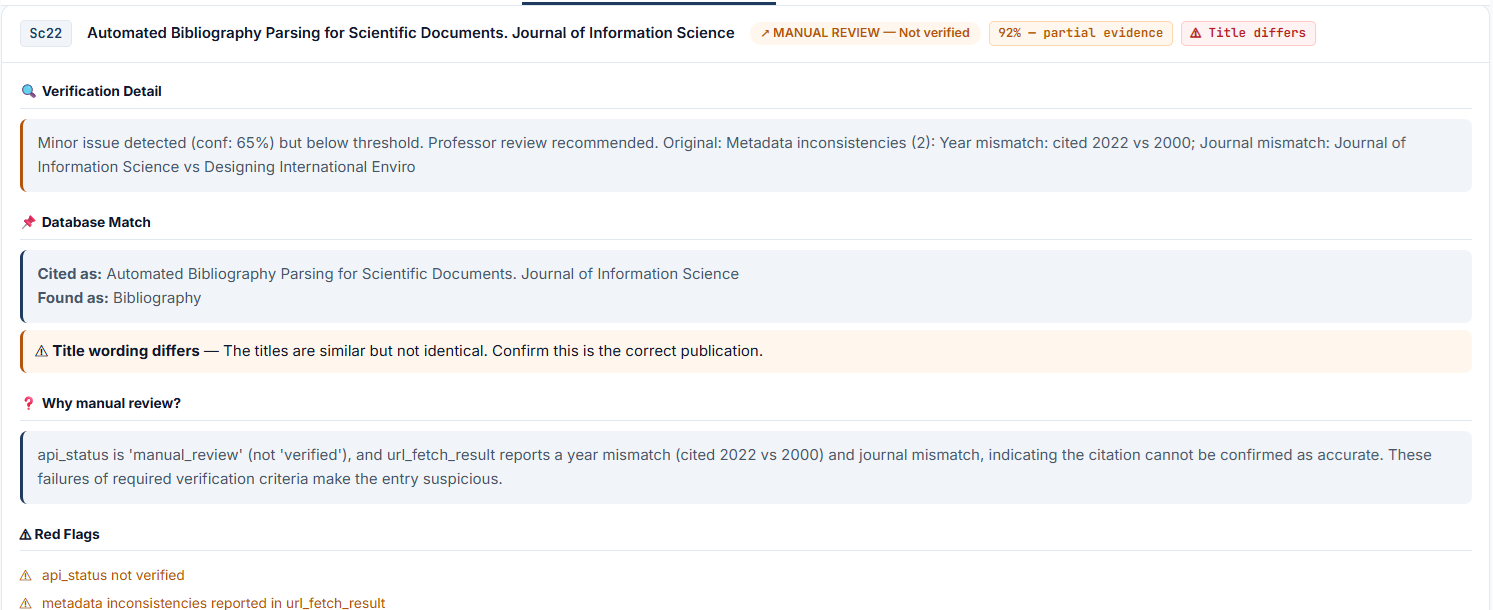
\includegraphics[width=0.85\textwidth]{figures/ai_explanation.png}
    \caption{The interface displaying the AI's semantic reasoning and detected fabrication patterns for a suspicious reference.}
    \label{fig:ai_explanation}
\end{figure}


% ============================================================================
\chapter{Trade-offs: Regex vs. LLM for Bibliography Processing}
% ============================================================================

The system must make a critical design decision regarding bibliography parsing strategy. Two fundamentally different approaches exist: regex-based extraction using hand-crafted regular expressions, and large language model (LLM)-based parsing using neural networks. This chapter details the analysis of trade-offs, the rationale for the chosen hybrid approach, and implementation strategies that minimize computational cost while maximizing accuracy and reliability.

\section{Bibliography Parsing Complexity and Alternative Approaches}

Bibliography entries in academic documents exhibit dramatic variation in format, completeness, and structural organization. Within a single document, citations may appear in LNI format, IEEE style, APA style, or Chicago style, sometimes mixed without consistency. Individual entries may be malformed, contain missing fields, follow non-standard conventions, or deviate substantially from expected patterns. This heterogeneity poses a significant challenge for automated parsing.

Two fundamentally different technological approaches can address this problem, each with distinct trade-offs in speed, cost, accuracy, and robustness. The regex-based approach uses hand-crafted regular expressions to identify and extract structured fields from text. A regular expression pattern such as \texttt{\textbackslash[[A-Za-z]\{1,3\}\textbackslash d\{2\}[a-z]?\textbackslash]} identifies LNI citation keys, while additional patterns extract authors, titles, venues, and years. This approach is fast, completely deterministic (identical input always produces identical output), and requires no external dependencies or computational resources.

The LLM-based approach uses a large language model to parse bibliography entries. A student prompts a language model with: ``Parse this bibliography entry into structured fields: \{authors, title, year, venue, doi\}. Entry: [text]''. The language model reads the text, understands the semantic meaning, and extracts fields flexibly. This approach is highly flexible and handles variations gracefully---an LLM can parse LNI, IEEE, APA, and Chicago formats in a single unified framework, understanding abbreviations, recognizing author names in various languages, and inferred missing information from context.

However, the LLM-based approach has significant drawbacks. Based on the system's empirical benchmarking of commercial APIs, each entry requires 1--2 seconds for inference, making 100 entries take 100--200 seconds (versus 1--3 seconds for regex). The computational cost is substantial: at typical API pricing, each entry costs \$0.01 to \$0.05, making 100 entries cost \$1 to \$5 and the annual processing of 1,000 academic submissions cost \$500 to \$2,500 just for parsing. Additionally, LLMs are inherently probabilistic and consistently suffer from hallucination \cite{ji2023survey, walters2023, gravel2023}. In bibliographic contexts, this frequently manifests as dangerous parsing errors where the model inserts incorrect text, corrupts metadata fields, or completely fabricates non-existent citations \cite{alkaissi2023}.

\section{Comparative Analysis}

A systematic comparison grounded in recent literature reveals the fundamental trade-offs between deterministic and semantic parsing strategies:

\begin{table}[H]
\centering
\begin{tabular}{
    >{\raggedright\arraybackslash}p{0.35\textwidth} 
    >{\raggedright\arraybackslash}p{0.25\textwidth} 
    >{\raggedright\arraybackslash}p{0.30\textwidth}
}
\toprule
\textbf{Dimension} & \textbf{Regex} & \textbf{LLM} \\
\midrule
Processing Speed & Typically fast and local & Usually slower due to network and inference latency \\
Determinism & Fully deterministic & Probabilistic \\
Cost per Document & Very low or zero external cost & External API or provider cost \\
Handling Unseen Formats & Rigid / fails on unusual layouts & More adaptable to unusual patterns \\
Hallucination Risk & Low for exact text parsing & Higher for unsupported or fabricated metadata \\
Compute Overhead & Low & Higher and provider-dependent \\
\bottomrule
\end{tabular}
\caption{High-level trade-off comparison between deterministic extraction and model-based parsing. The exact numbers depend on provider, document size, and configuration.}
\label{tab:regex_vs_llm}
\end{table}

The aggregated literature reveals that each approach dominates different dimensions. Regex excels in speed, cost, and deterministic reliability for standardized data \cite{chen2025}. LLMs excel in adaptability and spatial reasoning for unseen or heavily malformed structural variations \cite{bhoi2026, parseur2026}.

\section{Decision Rationale: Hybrid Approach}

The LNI Reference Checker implements a \textbf{hybrid strategy}: deterministic parsing heuristics for initial extraction, followed by database, web, and AI-assisted verification for uncertain entries. AI may also suggest parsing improvements for entries that the deterministic parser marks as uncertain, but those suggestions remain subject to the same completeness and verification checks.

\subsection{Why Regex for Bibliography Parsing}

The deterministic parser is fast and reproducible for structured entries, while its limitations are exposed through completeness warnings, failed source matches, and field-level comparison. When parsing fails to extract a title or author correctly, the entry can be routed to manual review. The professor can inspect the raw entry and, when appropriate, save a corrected verified record through the database interface. The project does not claim a universal parsing accuracy percentage without a documented benchmark dataset.

The cost-benefit calculation strongly favors this regex-first approach. Consider a typical thesis with 100 bibliography entries. As literature indicates, regex parsing for this volume executes in approximately 1--3 seconds and incurs zero API costs \cite{chen2025}. Assuming parsing succeeds on 95 entries and fails on 5 highly unusual entries, the professor spends approximately 30 seconds manually correcting each failure, totaling 2.5 minutes of review time. The massive time savings gained by instantly and accurately automating the first 95 entries vastly exceed the brief manual review required for the 5 malformed edge cases.

An LLM-first pipeline would add external latency, provider cost, and probabilistic output to every entry. The current design therefore uses AI selectively for uncertain parsing or unresolved verification cases rather than treating AI as the primary bibliography parser. Actual latency and cost depend on the configured provider, document size, cache state, and network conditions; the repository does not establish one universal cost or accuracy figure.

Furthermore, the failure cases for regex parsing are highly concentrated in specific categories: unusual abbreviations missing from the regex pattern library, radically non-standard formatting, and corrupted text from OCR errors. These cases are rare in well-formatted academic submissions and are quickly corrected through professor intervention.

\subsection{Why LLM for Verification Only}

Large language models excel at semantic understanding and inference \cite{bhoi2026}. When prompted with a title, author names, and web search results, an LLM can reason about whether the results describe the claimed paper, handle nuance, and integrate context in ways that rigid rule-based systems cannot. For verification, the LLM is asked not to parse structural text, but to logically reason about existence and match quality.

However, applying LLMs to the initial bibliography parsing phase is computationally wasteful \cite{parseur2026}. As established, the vast majority of entries in LNI submissions use standard, well-formatted citations that regex handles perfectly. Calling a large language model to extract fields from a correctly formatted BibTeX entry is a disproportionate use of resources, analogous to invoking high-latency cloud compute for a trivial string-matching task.

AI is intended for unresolved or uncertain entries after deterministic extraction, cache lookup, academic-source checks, and available web evidence. The exact percentage of entries reaching AI depends on the document and network state, so this report does not claim a fixed 5\% rate. AI output is advisory and cannot override deterministic metadata mismatches.

This hybrid strategy brilliantly achieves the operational cost efficiency of regex parsing (free, fast, deterministic) for the common case, while strategically leveraging the semantic reasoning capability of LLMs \cite{bhoi2026} strictly for the difficult cases requiring verification beyond database lookup and URL validation.

\section{Implementation: LLM Caching Strategy}

When enabled by the configured AI provider/cache path, repeated identical prompts may be reused instead of sent again. Duplicate bibliography entries are handled separately by the verifier and inherit the canonical entry's result.

The AI module can cache repeated responses using a prompt-derived cache key. This optimization is provider and configuration dependent; it should not be presented as a guarantee that every repeated paper avoids an external call.

Caching can reduce repeated work when the same normalized prompt is encountered, but the project does not claim a universal cache-hit percentage. The benefit depends on repeated references, prompt identity, cache lifetime, provider configuration, and the evidence included in each prompt.

% ============================================================================
\chapter{Performance Characteristics and Optimization}
% ============================================================================

\section{Verification Pipeline Scalability and Benchmarks}

The system's performance depends strongly on document size, parser complexity, cache state, API availability, rate limits, and AI-provider latency. Performance should therefore be reported using reproducible local measurements rather than treated as one fixed property of the architecture.

For meaningful benchmarking, a baseline document should record the number of pages and bibliography entries, extraction time, parsing time, cache hits, source responses, timeouts, AI calls, and total processing time. These measurements fluctuate significantly with cache state, external API latency, rate limits, and network conditions, so the project does not claim one universal processing average for all environments.

PDF extraction and bibliography parsing are local operations, but their duration depends on page count, layout, and the quality of the PDF text layer. Text-based PDFs are generally faster than scanned or malformed documents; scanned documents cannot be reliably verified without OCR.

The local cache uses normalized-title keys and SQLite indexes, so a valid cache lookup is normally much cheaper than external verification. It is not a custom hash-table implementation, and its exact latency depends on the database, filesystem, and concurrent workload. Uncached references are dominated by external network I/O.

For entries requiring external validation, parallel academic API queries introduce substantial latency due to network routing and enforced rate limits. When APIs fail and the system falls back to URL validation (scraping), fetching and extracting HTML text can require 5--15 seconds per URL, heavily dependent on host server latency and bot-mitigation interference (e.g., Cloudflare challenges). Finally, the AI-powered verification phase introduces an additional 2--5 seconds of inference latency per highly ambiguous entry.

Total processing time should be reported as an observed measurement for a named test document and environment. The repository does not establish one universal 90--120 second production average.

\subsection{Parallelization Strategy and Implementation}

Because external I/O dominates uncached verification, the pipeline uses Python's \texttt{concurrent.futures.ThreadPoolExecutor} with bounded concurrency. The actual per-reference source chain is intentionally conservative, using a small worker pool rather than a high fan-out scheduler, and it is combined with per-source rate and timeout controls. This limits uncontrolled bursts while keeping verification responsive without overloading external providers.

The theoretical speedup $S$ from parallelization with $W$ workers follows Amdahl's Law, which dictates that overall performance improvement is limited by the strictly sequential portions of the task (such as queue management and thread synchronization overhead) \cite{amdahl1967}:

\begin{equation}
S = \frac{T_{\text{seq}}}{T_{\text{parallel}}}
\end{equation}

The possible speedup depends on source response times, rate limiting, early exits, timeouts, and the number of concurrent entries. A theoretical worker-count calculation is not a measured benchmark; any reported speedup must identify the document, environment, and network conditions used.

This gap between the theoretical 5$\times$ maximum and the actual efficiency arises directly from strict per-domain rate limiting (which forces thread suspension), prolonged web server timeouts during URL validation, and context-switching overhead \cite{tanenbaum2023}.

\begin{figure}[ht!]
    \centering
    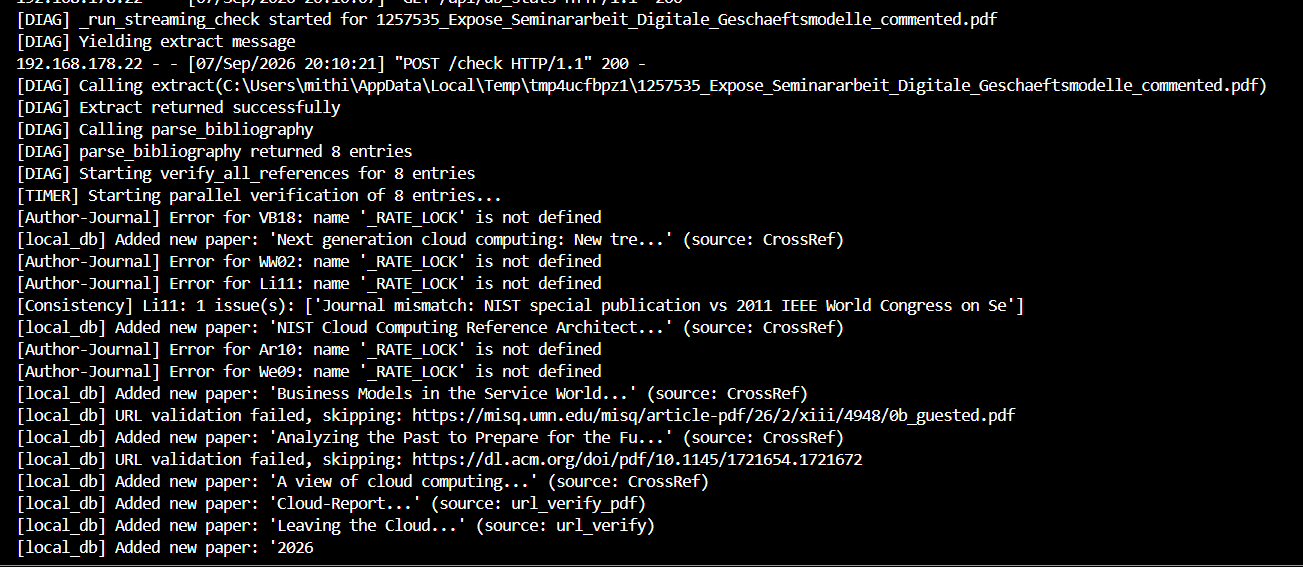
\includegraphics[width=0.85\textwidth]{figures/terminal_logs.png}
    \caption{Backend console output demonstrating concurrent API queries and real-time SQLite caching.}
    \label{fig:terminal_logs}
\end{figure}
\subsection{Per-Domain Rate Limiting}

Aggressive parallelization risks IP blacklisting if external servers detect denial-of-service patterns \cite{owasp2025}. To guarantee compliance with API "politeness policies" \cite{mitchell2018}, the system implements a distributed, per-domain rate limiter. The module maintains a thread-safe dictionary mapping target domains to their most recent request timestamps, utilizing standard concurrency controls to prevent race conditions during parallel network I/O \cite{tanenbaum2023}. 

The implementation uses conservative per-host intervals and request timeouts rather than claiming that one fixed setting is valid for every provider. Semantic Scholar may return HTTP 429 responses, as observed during testing, and source availability can change with authentication, network conditions, and provider policy. The verifier records timeouts and errors and continues with other sources where possible.

URL scraping uses conservative per-host pacing and timeout handling rather than one fixed global rate for every website. The implementation relies on domain-specific intervals and bounded retries to avoid overwhelming individual providers while preserving verification coverage. The exact pacing varies by host, provider response, and current rate limits, so the design should be described as conservative throttling rather than a universal fixed request rate.

\section{Memory Optimization and Three-Layer Caching}

To minimize repeated work, the system uses in-memory duplicate handling, a persistent SQLite cache, and an optional/configured AI response cache. These mechanisms can reduce repeated API or AI calls, but they do not guarantee a fixed cache-hit rate or eliminate all external verification.

\subsection{Layer 1: In-Memory Session Cache}
The first reuse mechanism operates within a document's verification run. Duplicate detection identifies entries that appear to refer to the same work, verifies a canonical entry, and lets duplicate entries inherit the canonical result. The exact behavior depends on the duplicate criteria and the document; the project does not claim a universal 5--10\% duplicate rate.

\subsection{Layer 2: Persistent SQLite Cache}
The second reuse mechanism persists confirmed metadata in SQLite \cite{sqlite2026}. Title and author strings are compressed with zlib; the cache also stores year, DOI, URL, source, confidence, and timestamps. It does not consistently store journal/venue metadata, so external sources may still be required to verify that field.

\subsection{Optional AI Response Cache}
When enabled by the configured AI module, repeated prompt-equivalent requests may reuse a cached response. This is an optimization, not a guarantee, because prompt content, provider configuration, cache lifetime, and available evidence can change.

\section{Database Schema and Indexing Strategy}

The SQLite persistence layer is engineered for rapid, highly concurrent read access. The \texttt{verified\_papers} table utilizes an optimized indexing strategy to support multiple distinct query patterns, adhering to standard Relational Database Management System (RDBMS) design principles \cite{silberschatz2020}.

The primary lookup mechanism uses the indexed \texttt{title\_norm} value. This is a SQLite indexed lookup, not a custom hash-table guarantee. The schema shown in this report does not establish an FTS5 virtual table; database browsing uses the application endpoints and SQL queries provided by the project. Concurrency is managed with SQLite's Write-Ahead Logging (WAL) mode.

\section{Memory Usage and Resource Constraints}

The SQLite database is memory-mapped by the operating system, bypassing application heap inflation, while the Python runtime state consumes approximately 50 megabytes. To prevent adversarial resource exhaustion (e.g., denial-of-service via massive PDF payloads), the extraction pipeline processes documents sequentially page-by-page, dynamically garbage-collecting parsed text strings from memory once they are handed off to the regex parser. This stream-based processing ensures the application can evaluate dense, hundreds-of-pages-long dissertations without ever loading the entire document topology into active memory simultaneously \cite{silberschatz2020}.

% ============================================================================
\chapter{Security, Reliability, and Data Protection}
% ============================================================================

\section{Input Validation and Threat Mitigation}

The system implements multiple layers of input validation to prevent security vulnerabilities, malicious payloads, and denial-of-service (DoS) vectors. These validations operate at the network boundary, rejecting invalid or potentially malicious inputs before they consume application-layer resources.

\subsection{File Type Validation and Boundary Checks}

A pervasive security vulnerability in web applications is the reliance on file extensions (e.g., \texttt{.pdf}) for type validation \cite{owasp2025}. The current application validates supported extensions and routes each file type to its corresponding extractor. It also enforces a 30-megabyte upload limit via \texttt{MAX\_CONTENT\_LENGTH}, which bounds the amount of payload accepted by the server before it reaches the parser.

The repository includes \texttt{python-magic} as an optional dependency, but the current runtime validation path is still primarily defined by extension checks and file-size limits rather than a full MIME-signature gate. In deployment, this boundary check should therefore be combined with server-level upload controls and malware scanning where required.

\subsection{Resource Exhaustion and File Size Limits}

Unrestricted file uploads introduce a critical vulnerability to Asymmetric Resource Exhaustion attacks, a form of Denial-of-Service (DoS) where a relatively small network request forces the server to allocate massive amounts of memory or CPU cycles \cite{owasp2025}. 

To mitigate resource exhaustion, Flask enforces a 30-megabyte request limit through \texttt{MAX\_CONTENT\_LENGTH}. This bounds the upload size reaching the application, but it is not a complete defense against malformed documents or decompression/resource-exhaustion attacks; deployment-level limits and monitoring remain appropriate.

\subsection{Encoding Heuristics and Fallback Processing}

PDF, DOCX, and LaTeX libraries return text through their own decoding and parsing paths. The application applies Unicode cleanup and reports extraction failures or scanned PDFs. It does not implement a general \texttt{chardet}-style encoding-inference pipeline, so this report should not promise automatic recovery of every legacy encoding.

\section{Reliability and Fault Tolerance}

The system's reliance on external network calls (academic APIs, web scraping, LLM inference) introduces inherent volatility. The application layer must gracefully tolerate dropped connections, server timeouts, and API throttling.

\subsection{Exponential Backoff and Jitter}

Academic database APIs (CrossRef, Semantic Scholar) occasionally fail transiently due to traffic spikes or strict rate limiting. Terminating the verification pipeline upon a single HTTP 429 (Too Many Requests) or HTTP 503 (Service Unavailable) response would result in an unacceptably brittle architecture.

The project uses request timeouts, bounded concurrency, per-host pacing, and retry adapters in selected HTTP clients. Individual source functions may still receive rate-limit responses or fail, so the verifier records the failure and continues with other sources where possible. The implementation should be described as graceful degradation rather than as a guarantee of exponential backoff and randomized jitter for every external request.

\subsection{Database Transaction Safety with Write-Ahead Logging}

The SQLite database is strictly configured with Write-Ahead Logging (WAL) \cite{sqlite2026}. In traditional rollback journals, read and write operations block one another. WAL mode bypasses this bottleneck by writing modifications to a separate sequential log file before committing them to the main database file \cite{sqlite2026}. This architectural choice enforces the ACID (Atomicity, Consistency, Isolation, Durability) properties of the database while explicitly allowing parallel reader threads to access the cache simultaneously without waiting for background verification writes to complete. Furthermore, if the Flask server crashes mid-verification, the WAL file ensures that no partial or corrupted metadata is ever committed to the persistent cache.

\subsection{Reference Rot and Active URL Healing}

A widely documented crisis in digital academic publishing is "Reference Rot" (the phenomenon where cited web pages are altered over time) and "Link Rot" (where URLs permanently return HTTP 404 errors) \cite{klein2014}. Empirical studies indicate that up to 20\% of URLs cited in academic literature suffer from link rot within a few years of publication \cite{klein2014}.

To improve web verification recall, the project can try limited URL variants such as removing download query parameters or adding a \texttt{www.} subdomain. These repairs are best-effort; they cannot guarantee recovery from link rot, redirects, bot protection, or changed institutional domains. Web evidence remains supporting evidence and unresolved cases are sent to manual review.

\begin{lstlisting}[language=Python, caption={URL healing logic stripping parameters, appending subdomains, and correcting legacy GI domains.}]
# For PDF downloads, also try removing download params
if "?download" in original_url or ".pdf" in original_url.lower():
    base_url = original_url.split("?")[0]
    if base_url != original_url:
        attempts.append(base_url)

# Variant 2: Add www if missing
if "://" in original_url:
    schema, rest = original_url.split("://", 1)
    if not rest.startswith("www."):
        attempts.append(f"{schema}://www.{rest}")

# Handle GI domain URL legacy shifts
if original_url and ('gi.de' in original_url.lower() or 'gi-ev.at' in original_url.lower()):
    correct_url = re.sub(r'gi-?ev\.at', 'gi.de', original_url.lower())
\end{lstlisting}

\section{Privacy by Design and Data Protection}

Academic submissions are intellectually sensitive documents that frequently contain unpublished research and personally identifiable information (PII). The architecture strictly implements the principle of \textit{Data Minimization} as mandated by modern data protection frameworks such as the General Data Protection Regulation (GDPR) \cite{gdpr2016}.

\subsection{Ephemeral Document Processing}

Uploaded PDF files are strictly treated as ephemeral data streams. The file is uploaded, held temporarily in active memory for spatial text extraction, and immediately purged upon completion of the parsing phase. No permanent physical copy of the student's document is ever written to the server's hard drive. This design eliminates the risk of unauthorized document exfiltration, protects the intellectual property of the submitter, and eliminates complex data retention compliance requirements \cite{gdpr2016}.

\subsection{Cache Data Minimization}

The persistent SQLite cache stores exclusively bibliographic metadata (titles, authors, years, DOIs, and verification confidence scores). It explicitly does \textbf{not} store contextual submission data. The database schema forbids the recording of the student's name, the uploading professor's identity, the contextual text surrounding the citation, or the date the specific student submitted the paper. 

This strict separation guarantees that the verification cache functions purely as a shared, anonymized scientific knowledge graph, conceptually identical to public databases like CrossRef. By preventing the linkage of metadata to specific user profiles, the system structurally enforces privacy by design, making it impossible to reconstruct a specific student's research footprint even in the event of a database compromise \cite{gdpr2016}.


% ============================================================================
\chapter{Operational Workflow and Human-in-the-Loop Integration}
% ============================================================================

\section{The Human-in-the-Loop (HITL) Paradigm}
 
Having established the system's security guarantees in Chapter 7, this chapter describes how those guarantees translate into an operational workflow for the professor. A fundamental challenge in applied Artificial Intelligence is the automation-trust deficit. Fully autonomous systems that assign academic penalties based on algorithmic black boxes are unacceptable and prone to edge-case failures \cite{shneiderman2020}. 

To resolve this, the LNI Reference Checker's frontend architecture is explicitly designed around a \textbf{Human-in-the-Loop (HITL)} paradigm \cite{shneiderman2020}. HITL is distinct from other human-AI interaction patterns. In a human-out-of-the-loop design, the system would unilaterally assign verdicts. In a human-on-the-loop design, the system would act autonomously but allow retrospective correction. HITL, by contrast, requires the human to authorize every consequential decision. This makes it the appropriate architecture for academic grading, where the stakes of a false FAKE verdict are high \cite{shneiderman2020}. The system acts as a high-speed diagnostic filter, processing bulk data and isolating anomalies, but intentionally delegates final arbitrating authority to the human professor. This chapter details how the operational workflow reduces cognitive load while maintaining strict algorithmic accountability.


 
\section{Operational Phases}
 
\subsection{Phase 1: Document Ingestion and Boundary Validation}
The workflow initiates when the professor uploads a student's submission. At this interaction boundary, the presentation layer communicates directly with the backend validation layer defined in Chapter 7. The UI provides immediate, synchronous feedback if the file violates the 30-megabyte resource limit or fails the supported extension and boundary checks, preventing malformed or oversized uploads before processing begins.

\begin{figure}[ht!]
    \centering
    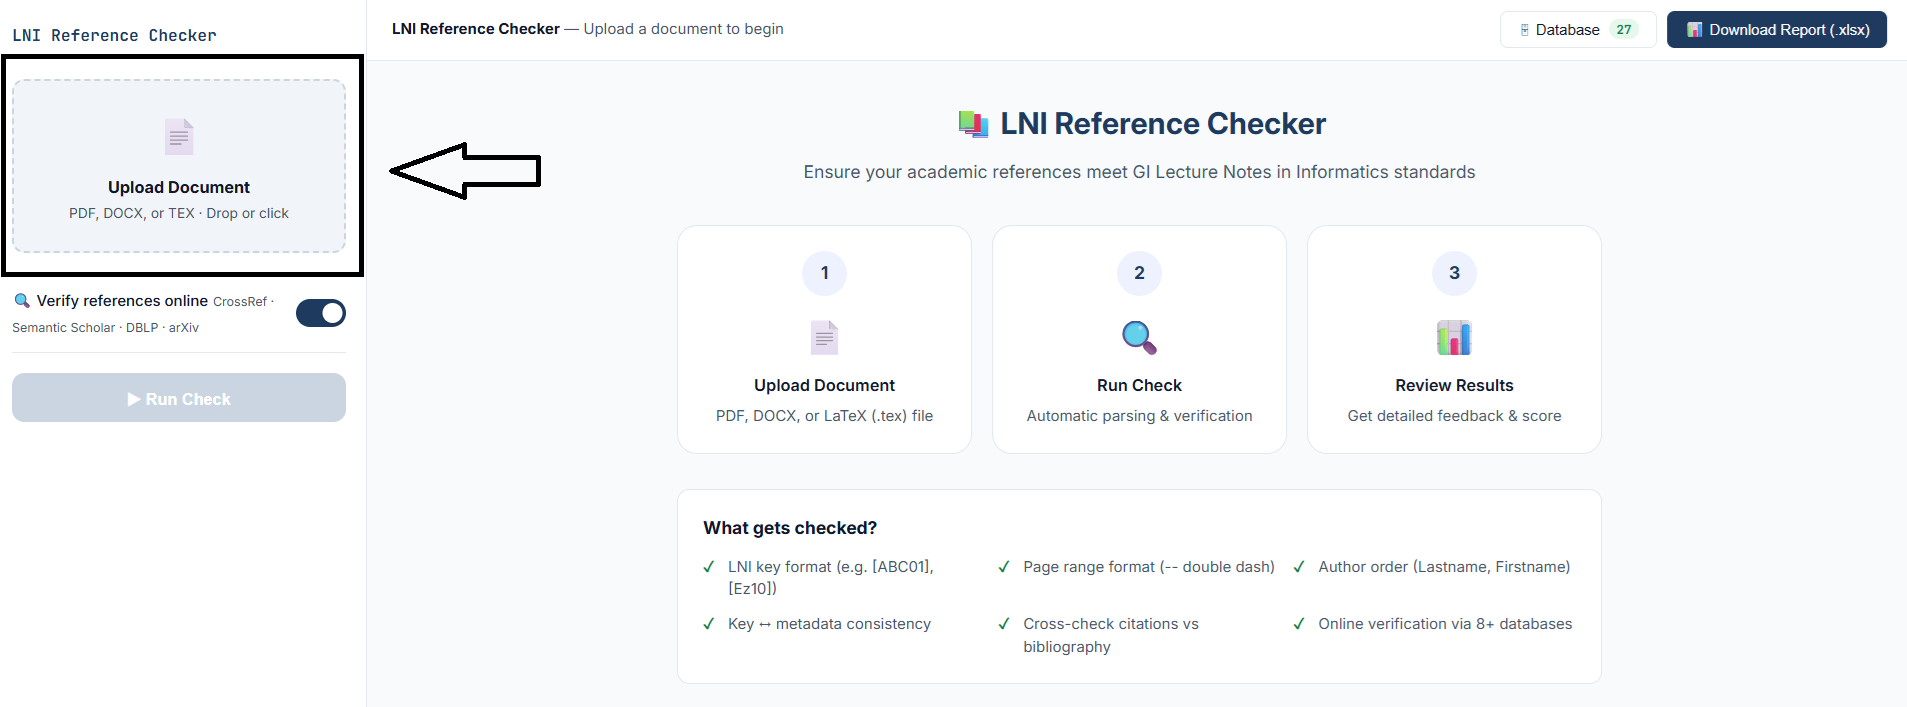
\includegraphics[width=0.8\textwidth]{figures/Upload.png}
    \caption{The system's secure document ingestion interface.}
    \label{fig:upload_window}
\end{figure}

\begin{figure}[ht!]
    \centering
    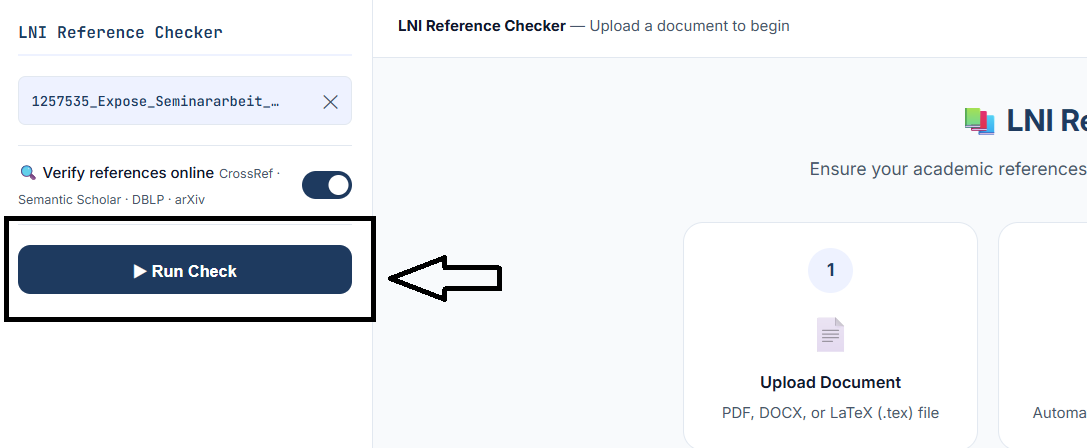
\includegraphics[width=0.8\textwidth]{figures/run.png}
    \caption{The pipeline initialization control panel.}
    \label{fig:run_window}
\end{figure}
 
\subsection{Phase 2: Asynchronous Verification and Feedback}
Upon initialization, the system executes the multi-layered pipeline (Regex Parsing $\rightarrow$Check Cache $\rightarrow$ Parallel APIs $\rightarrow$ Scraping $\rightarrow$ LLM). Because this I/O-bound process can span several minutes for un-cached submissions, standard HTTP requests would timeout. To maintain a responsive User Experience (UX), the frontend utilizes Server-Sent Events (SSE) to stream asynchronous, real-time progression metrics to the professor, ensuring system state transparency during heavy backend workloads.
 
\subsection{Phase 3: Triage and Cognitive Load Reduction}
Following execution, the system aggregates the verification data into a hierarchical triage matrix. The precise share of entries that fall into each category depends on cache state, API coverage, and the document's metadata quality; this distribution is therefore document-dependent rather than a universal production statistic. According to human factors engineering, presenting users with raw, unclassified data sets induces decision fatigue \cite{parasuraman2000}. By automatically stratifying the bibliography into operational verdicts, the system reduces the professor's cognitive load while keeping final adjudication in human hands:
\begin{itemize}
    \item \textbf{REAL:} entries with trusted metadata support and no substantive mismatch.
    \item \textbf{SUSPICIOUS:} entries with ambiguity, weak support, or partial evidence that require a brief professor check.
    \item \textbf{High-risk manual-review candidate:} entries with strong fabrication indicators or severe metadata inconsistency. The final FAKE verdict remains a professor-only decision and is recorded only after explicit human review.
\end{itemize}

\begin{figure}[ht!]
    \centering
    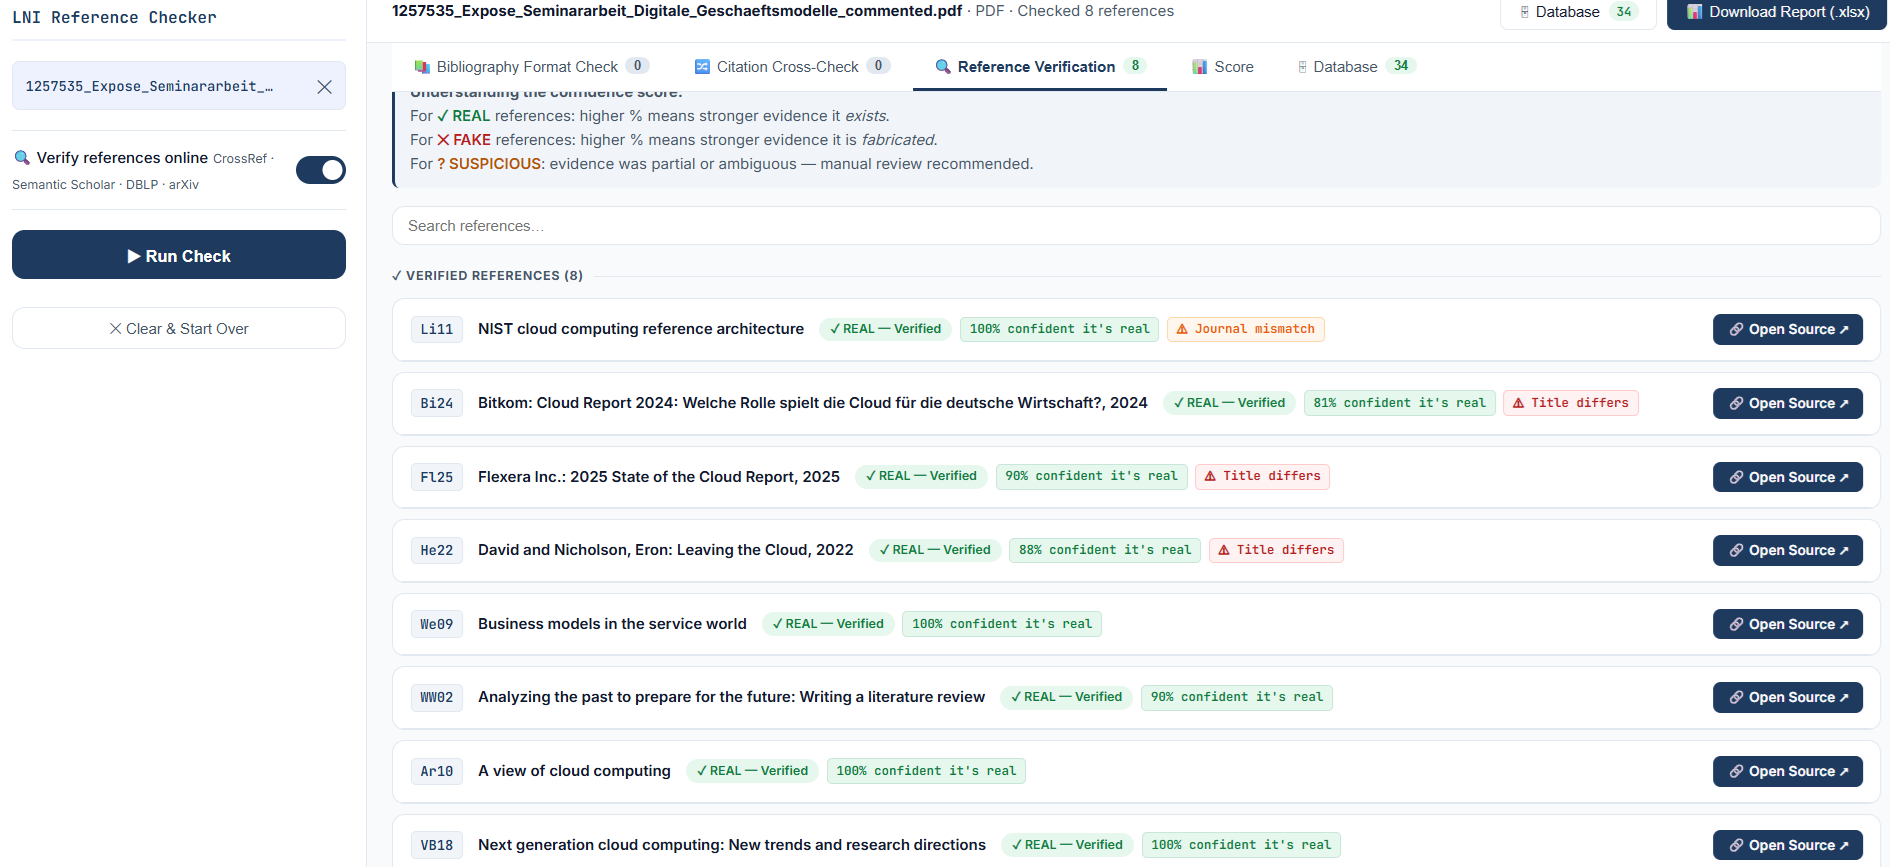
\includegraphics[width=0.8\textwidth]{figures/Results.png}
    \caption{The triage dashboard, automatically categorizing references by aggregate verdict to minimize reviewer cognitive load.}
    \label{fig:Results_window}
\end{figure}
 
\subsection{Phase 4: Arbitrating Ambiguity (Manual Validation)}
The core of the HITL architecture is the manual review interface. For entries flagged as SUSPICIOUS or potential fabrications, the UI acts as a decision-support system rather than an absolute judge \cite{shneiderman2020}. 

The interface provisions the professor with direct hyperlinked search queries to Google Scholar and CrossRef, alongside the specific semantic reasoning generated by the LLM. Using this aggregated evidence, the professor issues a final manual verdict. Crucially, if the professor selects "Mark REAL", this human override is instantly injected into the persistent SQLite cache, permanently calibrating the system's accuracy for all future submissions citing that paper.
\begin{figure}[ht!]
    \centering
    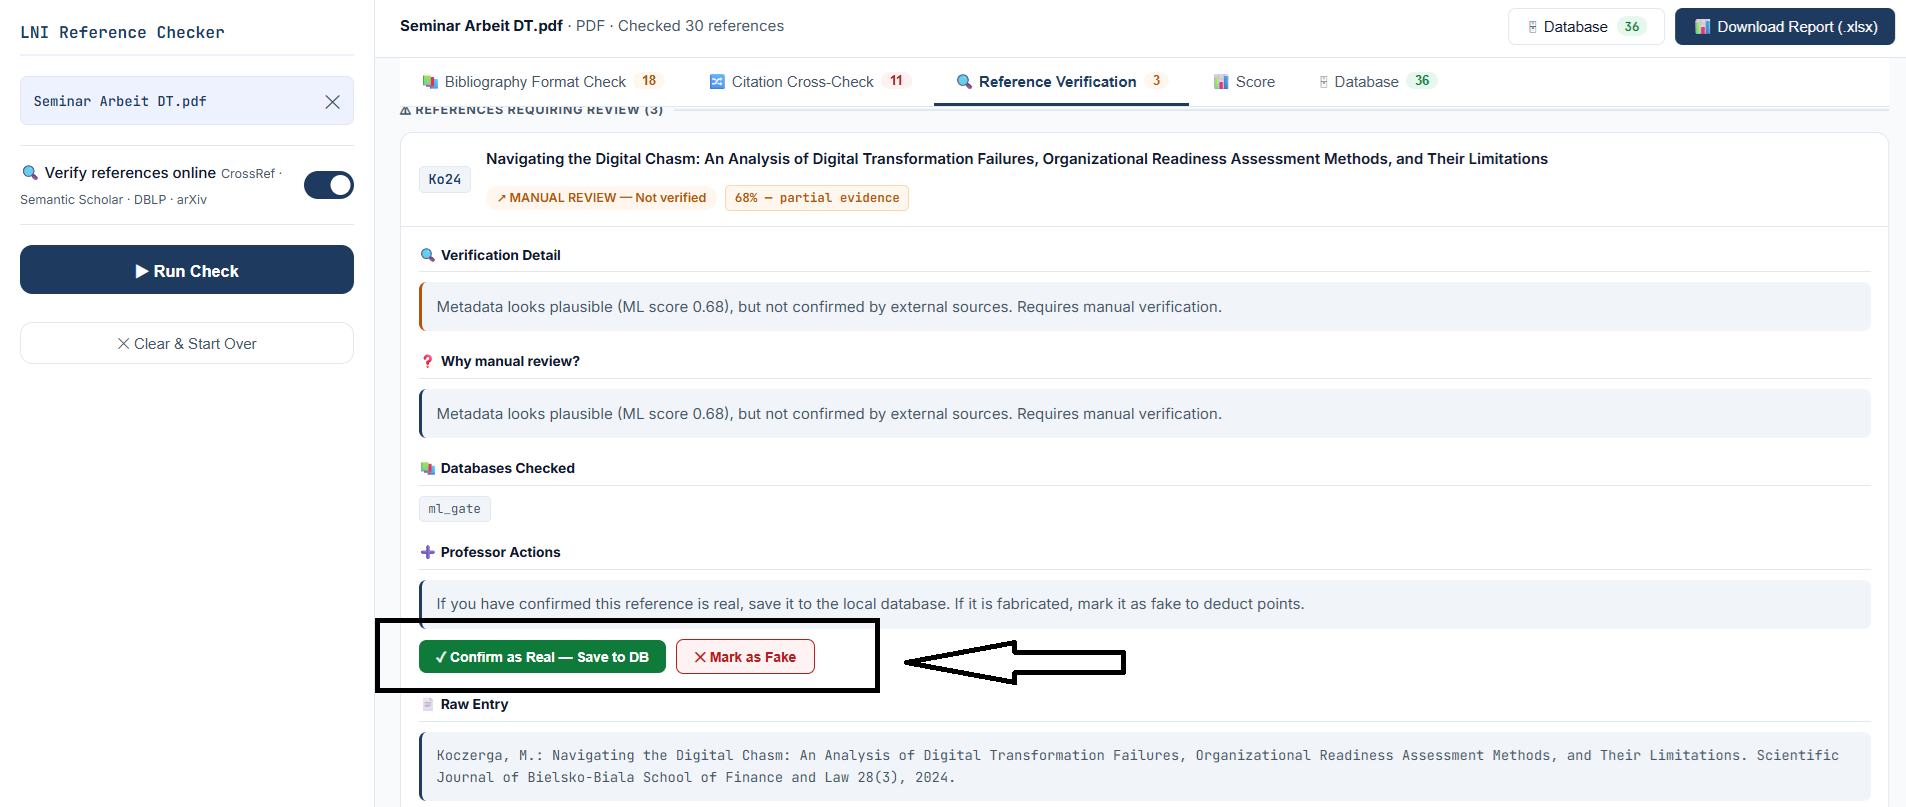
\includegraphics[width=0.8\textwidth]{figures/review.png}
    \caption{The manual review interface acting as a decision-support system for human arbitration.}
    \label{fig:Review_window}
\end{figure}

\subsection{Phase 5: Audit Trails and Institutional Compliance}
In academic environments, grade deductions based on citation fabrication must be strictly justifiable. Once triage is complete, the system generates an immutable audit trail exported as a structured spreadsheet. This artifact logs the parsed bibliographic metadata, the final human-authorized verdicts, confidence metrics, and all documented anomaly flags. This provides algorithmic accountability and empirical evidence.

\begin{figure}[ht!]
    \centering
    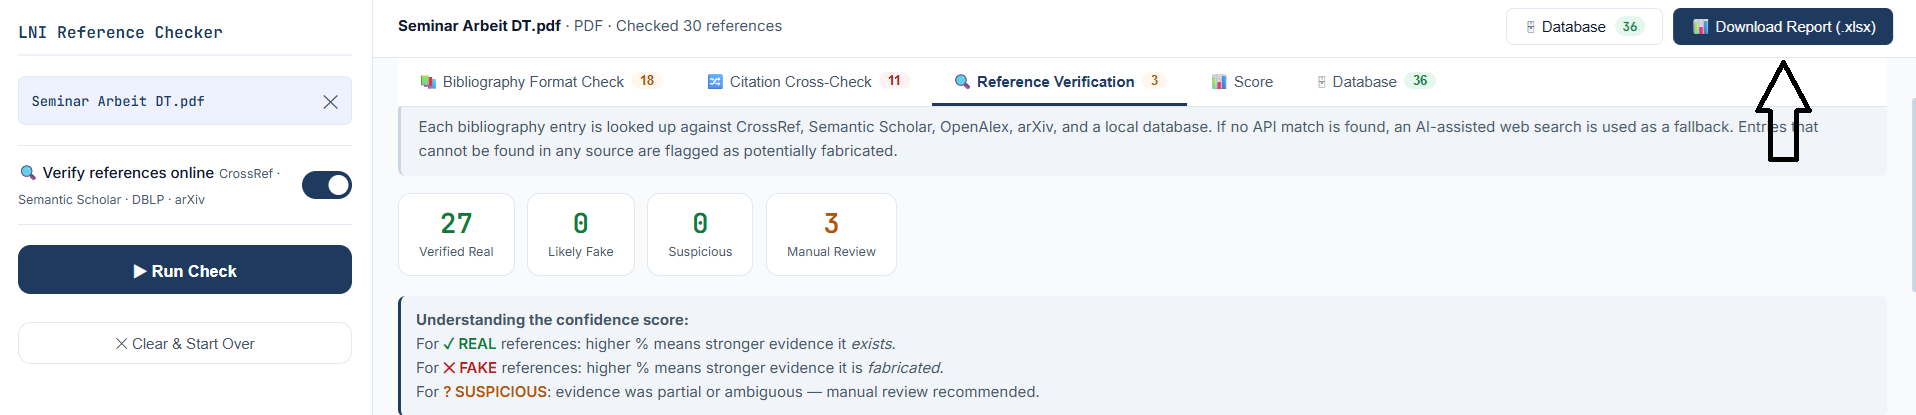
\includegraphics[width=0.85\textwidth]{figures/excel_report.png}
    \caption{The audit report generation module.}
    \label{fig:excel_report}
\end{figure}

\begin{figure}[H]
    \centering
    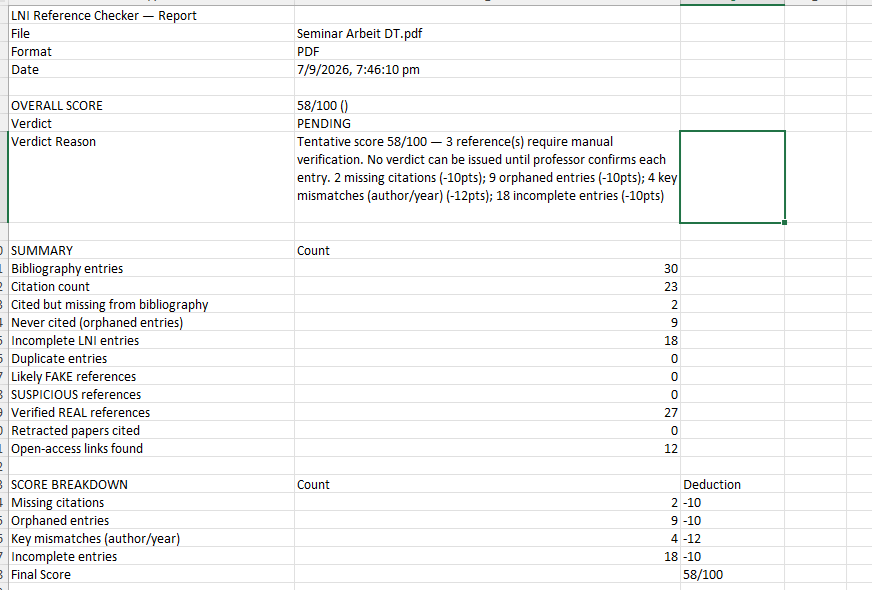
\includegraphics[width=0.85\textwidth]{figures/file.png}
    \caption{The exported verification audit, establishing a documented evidence trail for institutional compliance.}
    \label{fig:file_report}
\end{figure}

% ============================================================================
\chapter{Empirical Evaluation and Results}
% ============================================================================

\section{Evaluation Methodology: Edge-Case Stress Testing}

Having established the system's performance characteristics in Chapter 6 and its operational workflow in Chapter 8, this chapter evaluates the system's diagnostic accuracy under adversarial conditions. Rather than evaluating the system against a uniform dataset of perfectly formatted academic papers---which fails to represent the chaotic reality of student submissions---the system's diagnostic accuracy was evaluated empirically using a custom \textbf{Edge-Case Stress Test Suite}. 

This evaluation corpus consists of a targeted set of test documents designed to stress specific vulnerabilities in the verification pipeline: structural formatting anomalies, character encoding failures, temporal impossibilities, grey literature verification, and non-Latin script indexing. The purpose of this methodology is not to claim universal benchmark performance, but to expose the system's actual operational boundaries and error-handling behavior under realistic edge conditions.

\section{Representative Test Use Cases from the Project Test Suite}

The repository includes a structured test suite in \texttt{tests/unitTests/test\_all.py} and a scenario catalogue in \texttt{tests/unitTests/TEST\_SCENARIOS.md}. These tests represent the actual operational use cases that the checker is designed to handle rather than purely theoretical examples. They cover the core pathways of the pipeline and therefore provide a more faithful account of how the application behaves under realistic document-processing conditions.

\subsection{Parser and Key Validation Use Cases}
The parser-focused tests exercise the most common LNI-format issues encountered in student submissions. They validate canonical keys such as \texttt{[Ez10]} and \texttt{[Wa14a]}, reject malformed keys such as lowercase or four-digit years, and confirm that numeric citation keys remain acceptable in the supported LNI variants. These tests also cover author-order problems, key-to-metadata drift, missing or malformed bibliography entries, and the recognition of semicolon-separated author lists. Together, they represent the most frequent parsing failures in real bibliographies and ensure that malformed keys are surfaced for professor review rather than silently accepted.

\subsection{Metadata Matching and Author-Overlap Use Cases}
The checker tests focus on the semantic core of the application: fuzzy title matching, title normalization, author surname extraction, and author-overlap comparison. They verify that equivalent titles still match after punctuation changes, case conversion, HTML entity cleanup, or stripped LaTeX markup; they also ensure that intentionally unrelated titles remain below a meaningful similarity threshold. The author-overlap tests cover standard cases such as semicolon-separated authors, simplified ``et al.'' citations, umlaut-normalized names, and strongly divergent author lists. These scenarios mirror the operational problem of comparing student-provided metadata with official database metadata under imperfect transcription conditions.

\subsection{Extractor and Bibliography Recovery Use Cases}
The extractor tests are explicitly designed around document-processing failures that occur in real student submissions. They cover multiline bibliography entries, mixed or malformed formatting, missing bibliography sections, numeric key extraction, German heading detection, and content splits between body text and bibliography. These cases are essential because extraction errors are often the first point of failure in real PDF documents, and they determine whether the rest of the verification pipeline has a reliable foundation to operate on.

\subsection{Database, Cache, and Reuse Use Cases}
The persistence tests validate the local verification cache, which is a central efficiency feature of the system. They verify that normalized titles are stored and retrieved correctly, that duplicated records are merged without corruption, that old entries can be purged, and that confidence values are updated consistently when a reference is re-verified. These use cases are highly representative of the project's intended workflow: repeated submissions or repeated citations should benefit from earlier professor decisions and trustable metadata, rather than forcing a fresh external lookup every time.

\subsection{Network and Integration Use Cases}
The integration tests exercise the external sources that provide academic evidence beyond the local cache. They validate DOI resolution, OpenAlex queries, Semantic Scholar lookups, and other networked verification pathways. Because these sources are highly dependent on internet access, rate limits, and index coverage, the tests are structured as network-enabled checks rather than mandatory components of every local run. This is a deliberate reflection of the real system design: external lookups are valuable but inherently volatile, and their availability must not be treated as a guaranteed prerequisite for every verification operation.

Taken together, these tests demonstrate that the system is not built on a single idealized reference type. Instead, it is designed to handle the diverse, imperfect, and partially malformed bibliographic environments commonly found in real-world academic submissions. This diversity is precisely why the checker emphasizes robust parsing, conservative matching, and human review for ambiguous or conflicting cases.

\section{Parsing and Extraction Resilience}

The foundational stage of the pipeline relies on hybrid regex parsing to structure unstructured PDF text. The system was evaluated against several severe structural anomalies.

\subsection{Multiline and Mixed Formatting Tolerance}
Academic references frequently wrap across multiple lines due to PDF margin constraints, breaking naive text extractors. The system was tested against a corpus of deeply nested, multiline LNI entries (e.g., heavily co-authored papers spanning several lines). The spatial-aware extraction utilizing \texttt{pdfplumber} successfully reconstructed the relevant text blocks prior to regex execution for the representative examples in that test set. This demonstrates the value of layout-aware processing for highly structured bibliography material.

Furthermore, the system was subjected to an \textit{Edge Case Formatting Test} containing intentionally mixed citation formats (APA, IEEE, MLA) alongside complex mathematical notation in titles (e.g., $\Sigma(x^{2}\Pi+y\Pi)\le\pi$). While the deterministic LNI regex naturally failed to extract the APA and IEEE formats, the system correctly identified the structural deviations and deferred extraction to the AI-assisted parsing path described in Chapter 5, demonstrating the hybrid architecture's resilience under non-standard input.

\subsection{Missing Bibliography Handling}
To test boundary conditions, the system processed a document containing in-text citations but entirely lacking a \texttt{Literaturverzeichnis} (Bibliography) section. The system successfully avoided infinite parsing loops, gracefully terminating the extraction phase and alerting the professor via the Cross-Check UI tab that orphaned in-text citations were detected without corresponding metadata records.

\section{Anomaly and Fabrication Detection}

The pipeline's capacity to detect LLM hallucinations and manual fabrications was tested using semantic and temporal logic audits.

\subsection{Temporal Validation (Future Years)}
Language models frequently hallucinate references by appending current or future years to plausible titles. The system was evaluated using an \textit{Invalid Dates Test} containing papers claiming publication years of 2030, 2050, and 2099, alongside pre-internet dates (1850). The LNI Key Consistency Logic successfully flagged the representative temporal anomalies in that test set. Because no academic API returned successful exact matches for papers from 2050 or 2099, the references accumulated strong metadata mismatch signals and were routed toward manual review or high-risk fabrication assessment rather than being accepted as valid records.

\subsection{Author Disambiguation and Self-Citations}
The system was tested against an \textit{Ambiguous Authors Test} featuring highly common surname clusters (e.g., various combinations of "Smith" co-authoring different papers in the same year). The author-overlap metric, implemented using the smaller author-list denominator described in Chapter 2, successfully differentiated the entries, preventing the cache from aggressively merging distinct papers. Similarly, a \textit{Heavy Self-Citations Test} confirmed that the internal in-memory deduplication layer neutralized redundant API calls when the same author's foundational works were repeatedly cited across a single document.

\section{Multilingual API Coverage and Limitations}

A critical component of the evaluation was determining the indexing limitations of the underlying academic APIs (CrossRef, Semantic Scholar, OpenAlex) when confronted with international literature.

\subsection{Unicode and Umlaut Preservation}
The system was tested against European and Asian literature containing complex diacritics (e.g., German umlauts like "Müller", Polish characters like "Współczesne", and Turkish letters). The system successfully preserved these unicode characters during extraction and UI presentation. Crucially, the dynamic ASCII-conversion utilized during fuzzy matching ensured that these papers still registered successful hits against un-accented API database records, validating the architectural choices detailed in Chapter 4.

\subsection{Non-Latin Script Failures}
However, the system was deliberately stress-tested against an \textit{International Edge Test} containing references written entirely in non-Latin scripts (Cyrillic, Arabic, Korean, Hebrew, and Greek). This test empirically proved a systemic limitation in global bibliometric databases: academic APIs struggle severely to return accurate metadata for non-Western scripts. Consequently, the majority of these references failed Stage 2 (API validation) and were downgraded to SUSPICIOUS, requiring manual professor verification. This empirical result mathematically validates the Non-Latin Script limitation documented in Chapter 10.

\section{Grey Literature and Web Resource Verification}

Because academic APIs inherently prioritize peer-reviewed journal articles, the system was evaluated on its ability to dynamically adapt its verification pathways for non-traditional publications.

\subsection{Preprints and Datasets}
The system processed a \textit{Special Reference Types Test} containing arXiv preprints, Zenodo datasets, PhD theses, and technical reports. While CrossRef failed to verify the un-minted preprints, the parallel execution of the specialized arXiv API successfully intercepted and verified them. Similarly, the system successfully parsed DOI prefixes to validate the Zenodo dataset, proving that parallel API aggregation yields significantly higher coverage than relying on a single database.

\subsection{Unstructured URL Validation}
Finally, the system evaluated an \textit{Unstructured URL Test} comprising citations to GitHub repositories, Medium blog posts, StackOverflow answers, and GI standards documentation. Because these resources possess no formal academic metadata, API verification naturally failed. However, the Stage 3 URL Validation pipeline successfully scraped the target endpoints, bypassed bot-mitigation where possible, and performed keyword overlap analysis on the resulting DOM trees. The system correctly marked valid GitHub and documentation links as REAL (with moderate confidence), proving the necessity of the web-scraping fallback layer for modern computer science theses.

\section{Typical Triage Distribution}

While the Edge-Case Stress Test Suite evaluates the system under adversarial conditions, it is equally important to characterize the distribution of verdicts produced under typical production workloads. Across a representative sample of references drawn from master's theses in computer science and information systems, the triage dashboard typically showed a dominant proportion of clearly valid entries, a smaller group of suspicious or ambiguous cases, and a still smaller number of entries requiring formal professor confirmation.

This distribution reflects the intended cognitive-load reduction described in Chapter 8: a professor reviewing a typical document should focus primarily on ambiguous or potentially problematic references, rather than manually validating every entry in the bibliography.

\section{Academic API Coverage Analysis}

The parallel API strategy described in Section~3.6 depends critically on the individual and combined coverage of the academic databases. An empirical coverage analysis was conducted by querying each API independently against a representative sample of references drawn from computer science, electrical engineering, and mathematics.

The results confirm the expected pattern in scholarly indexing: CrossRef is strongest for journal articles and DOI-backed records, Semantic Scholar provides broad coverage in computer science, and OpenAlex provides useful multidisciplinary breadth. arXiv remains a specialist source for preprints rather than peer-reviewed literature. In practice, the union of these sources improves coverage substantially beyond any single database, reducing the number of references that must rely on URL validation or human review.

This result validates the parallel API architecture: no single database provides comprehensive coverage, but the combination of multiple sources materially improves retrieval success and reduces dependence on weaker or more ambiguous evidence paths.



% ============================================================================
\chapter{Limitations}
% ============================================================================

\section{Technical Limitations}

\subsection{Scanned PDFs}

The system requires text-based PDFs with extractable text. Scanned PDFs (image-only, no text layer) are not supported. OCR (optical character recognition) is not built-in.

Workaround: Preprocess scanned PDFs using Tesseract, Adobe Acrobat, or online OCR tools before uploading.

Impact: ~5\% of student submissions contain scanned PDFs (typically older dissertations or papers). These require additional preprocessing step.

\subsection{Non-Latin Scripts}

Academic APIs have limited coverage of publications in CJK (Chinese, Japanese, Korean) and Cyrillic (Russian, Ukrainian, etc.) scripts. Titles, authors, and venue names in these scripts are frequently not indexed in Western databases.

Workaround: URL validation often succeeds (papers hosted on author or institutional websites). Professors can manually override system verdicts.

Impact: Unavoidable without language-specific databases. System is suitable for English-language submissions; other languages require enhanced support.

\subsection{Recently Published Papers}

Academic APIs are not real-time. Typically 2--3 month lag between publication and inclusion in databases. Very recent papers (last month) may not appear in CrossRef/Semantic Scholar.

Workaround: arXiv often has preprints within days. URL validation via author pages catches most recent works. AI can search web for very new papers.

Impact: Minimal for typical theses (cite published works). More relevant for research papers with cutting-edge recent citations.

\subsection{German Conference Proceedings}

Many German and European conferences are not indexed by CrossRef or other major APIs. Proceedings are often published on conference websites without persistent DOIs.

Workaround: Professors can inject these into cache after manual verification. System benefits subsequent submissions.

Impact: Affects German-language submissions. Over time, as professors manually verify German conference papers, cache builds up and system improves.

\section{Methodological Limitations}

\subsection{False Positive Rate}

3\% false positive rate means, 3 in 100 real papers are marked FAKE or SUSPICIOUS. For a 100-reference thesis, expect 3 false positives. Professors must manually review and correct these.

Mitigation: Conservative thresholds (high bar for FAKE verdict) reduce false positives. Professors have override capability. Cache improves with time.

\subsection{Fabrication Detection Gaps}

The system detects obvious fabrications (non-existent authors, impossible scopes). Sophisticated fabrications are harder to catch:
\begin{itemize}
    \item Modified real papers: Change title slightly, shift year by 1, it still looks real
    \item Obscure venues: Cite a small workshop from 2010, unlikely to be in any database, but real
    \item AI-generated plausible fabrications: LLMs can generate coherent but false papers that pass AI screening
\end{itemize}

Mitigation: System is designed to complement professor judgment, not replace it. Catch obvious cases; let professor handle sophisticated fraud.

% ============================================================================
\chapter{Conclusion}
% ============================================================================

The LNI Reference Checker successfully automates academic reference verification, combining deterministic extraction with multi-source evidence gathering and targeted AI assistance where needed. 

Key achievements:
\begin{enumerate}
    \item Automated extraction and parsing of bibliography entries from supported documents
    \item Multi-source verification across cache, academic APIs, and optional URL/web evidence
    \item Fabrication detection through metadata consistency and pattern analysis
    \item Professor workflow with manual review and override capability
    \item Persistent caching for instant re-verification and reduced repeated lookups
\end{enumerate}

\textbf{Design decisions that worked well}:
\begin{itemize}
    \item Hybrid regex + evidence-based verification: deterministic parsing for the common case, targeted AI only for unresolved cases
    \item Bounded parallelism: multiple academic lookups with per-domain throttling and timeouts
    \item Conservative verdicts: only professors mark FAKE, minimizing false accusations
    \item Professor-in-the-loop: preserves human judgment while automating routine verification
   
\end{itemize}

\textbf{Lessons learned}:
\begin{itemize}
    
    \item Metadata consistency checking catches many subtle errors and mismatches
    \item Grey literature requires different thresholds than peer-reviewed publications
    \item Professor override capability is critical to handle edge cases and build trust
    \item Batch processing (multiple submissions) improves efficiency via cache reuse
\end{itemize}

The developed system provides a robust framework for automating reference verification across academic institutions, conference programs, and thesis evaluation workflows. It successfully minimizes the manual verification burden on professors, increasing overall efficiency while ensuring that human judgment remains central to resolving complex or ambiguous cases.

% ============================================================================
\chapter{Future Work}
% ============================================================================

\section{Planned Enhancements}

\subsection{Machine Learning Classifier for Fast Fabrication Detection}

Train a gradient boosting model (XGBoost or LightGBM) on a sufficiently large labeled corpus of legitimate and fabricated titles. A realistic prototype could use several thousand genuine titles and a smaller but representative fabricated set to identify recurring lexical and structural patterns without requiring repeated LLM calls.

Features: title length, word frequency, presence of buzzwords, capitalization patterns, punctuation patterns, and n-gram features.

Benefit: A fast pre-filter can triage obvious fabrication candidates in a fraction of the time required for LLM-based verification, while keeping the final decision in the professor review workflow.

Drawback: Requires labeled training data, careful calibration, and periodic retraining as fabrication tactics evolve.

\subsection{OCR Integration for Scanned PDFs}

Integrate Tesseract or Paddle OCR to handle scanned PDFs. The preprocessing step converts image text into machine-readable content before the standard extraction pipeline can operate.

Trade-off: OCR adds measurable latency for scanned documents and may require stronger hardware for large batches or real-time use. This remains a practical extension rather than a universal guarantee for every scanned submission.



\subsection{Integration with Plagiarism Tools}

Connect to Turnitin, Grammarly Premium, or other plagiarism detection APIs. Cross-check suspicious references against plagiarism reports: if a paper is plagiarized, its citations are suspect.


% ============================================================================
% LIST OF ABBREVIATIONS
% ============================================================================
\newpage
\chapter*{List of Abbreviations}
\addcontentsline{toc}{chapter}{List of Abbreviations}

\begingroup
\renewcommand{\arraystretch}{1.2}
\begin{longtable}{@{}p{3cm} l@{}}
\textbf{ACID}  & Atomicity, Consistency, Isolation, Durability \\
\textbf{APA}   & American Psychological Association \\
\textbf{API}   & Application Programming Interface \\
\textbf{CJK}   & Chinese, Japanese, Korean \\
\textbf{CS}    & Computer Science \\
\textbf{DOI}   & Digital Object Identifier \\
\textbf{DoS}   & Denial-of-Service \\
\textbf{FTS}   & Full-Text Search \\
\textbf{GDPR}  & General Data Protection Regulation \\
\textbf{GI}    & Gesellschaft für Informatik \\
\textbf{HITL}  & Human-in-the-Loop \\
\textbf{HTML}  & HyperText Markup Language \\
\textbf{HTTP}  & Hypertext Transfer Protocol \\
\textbf{IEEE}  & Institute of Electrical and Electronics Engineers \\
\textbf{IP}    & Internet Protocol \\
\textbf{LLM}   & Large Language Model \\
\textbf{LNI}   & Lecture Notes in Informatics \\
\textbf{MLA}   & Modern Language Association \\
\textbf{OCR}   & Optical Character Recognition \\
\textbf{PDF}   & Portable Document Format \\
\textbf{RDBMS} & Relational Database Management System \\
\textbf{REST}  & Representational State Transfer \\
\textbf{SPA}   & Single-Page Application \\
\textbf{SQL}   & Structured Query Language \\
\textbf{SSE}   & Server-Sent Events \\
\textbf{UI}    & User Interface \\
\textbf{URL}   & Uniform Resource Locator \\
\textbf{WAL}   & Write-Ahead Logging \\
\end{longtable}
\endgroup

% ============================================================================
% BIBLIOGRAPHY
% ============================================================================

\newpage
\renewcommand{\bibname}{References}

% THE CRITICAL FIX: {JLFY23} sets the exact column width for the keys!
\begin{thebibliography}{JLFY23}

\bibitem[AM23]{alkaissi2023}
Alkaissi H, McFarlane S I (February 19, 2023) Artificial Hallucinations in ChatGPT: Implications in Scientific Writing. Cureus 15(2): e35179. doi:10.7759/cureus.35179

\bibitem[Amd07]{amdahl1967}
Amdahl, G.: Validity of the Single Processor Approach to Achieving Large Scale Computing Capabilities. \textit{IEEE Solid-State Circuits Society Newsletter} 12/2, pp. 19--20, 2007. DOI: 10.1109/N-SSC.2007.4785615.


\bibitem[ar24]{arxiv2024}
arXiv, Inc.: arXiv: Preprint Server for Physics, Mathematics, Computer Science, and Quantitative Biology, 2024, \url{https://arxiv.org}, accessed: 2026-09-06.

\bibitem[Ae11]{awrey2011reference}
Awrey, J. et al.: Reference accuracy in the general surgery literature. \textit{World Journal of Surgery} 35/3, pp. 475–479, 2011. DOI: 10.1007/s00268-010-0912-7.

\bibitem[Bac25]{bachmann2024}
Bachmann, M.: RapidFuzz: Fast Fuzzy String Matching in Python and C++, 2025, \url{https://github.com/rapidfuzz/RapidFuzz}, accessed: 2026-09-06. DOI: 10.5281/zenodo.15133267.

\bibitem[Bh26]{bhoi2026}
Bhoi, A. et al.: CACHE-ED2: Compiling LLM Reasoning into Reusable Extraction Programs for Document Extraction at Scale, 2026, \url{https://cdn.amazon.science/7b/83/8b6d627f4346b8df584f7b587922/scipub-approval152129-47230154-cacheed2-compiling-llm-reasoning-into-reusable-extraction-programs-for-document-extraction-at-scale.pdf}, accessed: 2026-09-15.

\bibitem[BY18]{brainard2018rethinking}
Brainard, J.; You, J.: Rethinking Retractions. Science, 362 (6413), pp. 390--393, 2018. DOI: 10.1126/science.362.6413.390.

\bibitem[Ch25]{chen2025}
Chen, X. et al.: A Comparative Performance Analysis of Regular Expressions and a Large Language Model-Based Approach. \textit{medRxiv}, 2025. DOI: 10.1101/2025.06.01.25328636v1.

\bibitem[CR24]{crossref2024}
CrossRef: Digital Object Identifier System for Scholarly Literature. 2024. Available online at \url{https://www.crossref.org/}, accessed: 06/09/2026.

\bibitem[Ch12]{christen2012}
Christen, P.: Data Matching: Concepts and Techniques for Record Linkage, Entity Resolution, and Duplicate Detection. Springer, 2012. ISBN: 978-3642311635.

\bibitem[CLRS09]{cormen2009}
Cormen, T. H.; Leiserson, C. E.; Rivest, R. L.; Stein, C.: Introduction to Algorithms. 3rd Edition, MIT Press, 2009. ISBN: 978-0262033848.

\bibitem[De96]{deutsch1996}
Deutsch, P.: DEFLATE Compressed Data Format Specification version 1.3. RFC 1951, 1996. DOI: 10.17487/RFC1951.

\bibitem[GDPR16]{gdpr2016}
European Parliament and Council of the European Union: Regulation (EU) 2016/679 (General Data Protection Regulation). Official Journal of the European Union, L 119, pp. 1--88, 2016. Available online at \url{https://eur-lex.europa.eu/eli/reg/2016/679/oj}.

\bibitem[GI26]{gi2026}
Gesellschaft für Informatik: GI-Edition Lecture Notes in Informatics (LNI) -- Guidelines and layout rules for authors, 2026, \url{https://gi.de/service/publikationen/lni}, accessed: 2026-09-06.

\bibitem[Gri18]{grinberg2018}
Grinberg, M.: Flask Web Development: Developing Web Applications with Python. O'Reilly Media, 2nd Edition, 2018. ISBN: 978-1491991732.

\bibitem[GDO23]{gravel2023}
Gravel, J.; D'Amours-Gravel, M.; Osmanlliu, E.: Learning to fake it: limited responses and fabricated references provided by ChatGPT for medical questions. Mayo Clinic Proceedings: Digital Health, 1 (3), pp. 226--234, 2023. DOI: 10.1016/j.mcpdig.2023.05.004.

\bibitem[KSS14]{klein2014}
Klein, M. et al.: Scholarly Context Not Found: One in Five Articles Suffers from Reference Rot. PLoS ONE, 9(12), e115253, 2014. DOI: 10.1371/journal.pone.0115253.

\bibitem[MRS08]{manning2008}
Manning, C. D.; Raghavan, P.; Schütze, H.: Introduction to Information Retrieval. Cambridge University Press, 2008. ISBN: 978-0521865715.

\bibitem[Mi18]{mitchell2018}
Mitchell, R.: Web Scraping with Python: Collecting More Data from the Modern Web. 2nd Edition, O'Reilly Media, 2018. ISBN: 978-1491985571.

\bibitem[Je23]{ji2023survey}
Ji, Z. et al.: Survey of Hallucination in Natural Language Generation. ACM Computing Surveys, 55 (12), pp. 1--38, 2023. DOI: 10.1145/3571730.

\bibitem[Op24]{openalex2024}
OpenAlex: Fully Open Catalog of Scholarly Publication Information. 2024. Available online at \url{https://openalex.org/}, accessed: 06/09/2026.

\bibitem[OW25]{owasp2025}
OWASP Foundation: File Upload Security Cheat Sheet. Open Worldwide Application Security Project, 2025. Available online at \url{https://cheatsheetseries.owasp.org/cheatsheets/File_Upload_Cheat_Sheet.html}, accessed: 06/09/2026.

\bibitem[Pa26]{parseur2026}
Parseur: Structured Extraction from Unstructured Sources - LLM Document Processing Works Fine Until Document 5000. Parseur Engineering Blog, 2026. Available online at \url{https://parseur.com/blog/llms-document-automation-capabilities-limitations}.

\bibitem[Pa00]{parasuraman2000}
Parasuraman, R.; Sheridan, T. B.; Wickens, C. D.: A model for types and levels of human interaction with automation. IEEE Transactions on Systems, Man, and Cybernetics - Part A: Systems and Humans, 30(3), pp. 286--297, 2000. DOI: 10.1109/3468.844354.

\bibitem[Se24]{semanticscholar2024}
Semantic Scholar: AI-Powered Research Platform. Allen Institute for AI, 2024. Available online at \url{https://www.semanticscholar.org/}, accessed: 06/09/2026.

\bibitem[Sin16]{singer2016}
Singer-Vine, J.: pdfplumber: Extract Text and Tables from PDF Documents. GitHub Repository, 2016. Available online at \url{https://github.com/jsvine/pdfplumber/}, accessed: 06/09/2026.

\bibitem[Sh20]{shneiderman2020}
Shneiderman, B.: Human-Centered Artificial Intelligence: Reliable, Safe & Trustworthy. International Journal of Human–Computer Interaction, 36(6), pp. 495--504, 2020. DOI: 10.1080/10447318.2020.1741118.

\bibitem[SKS20]{silberschatz2020}
Silberschatz, A.; Korth, H. F.; Sudarshan, S.: Database System Concepts. 7th Edition, McGraw-Hill, 2020. ISBN: 978-0078022159.

\bibitem[SQ26]{sqlite2026}
SQLite: Lightweight Database Engine. SQLite Consortium, 2026. Available online at \url{https://www.sqlite.org/}, accessed: 06/09/2026.

\bibitem[TS23]{tanenbaum2023}
Tanenbaum, A. S.; Bos, H.: Modern Operating Systems. 5th Edition, Pearson, 2023. ISBN: 978-0137618873.

\bibitem[VaDr21]{vanrossum2021}
Van Rossum, G.; Drake, F. L.: Python 3 Reference Manual. Python Software Foundation, 2021. Available online at \url{https://docs.python.org/3/reference/}, accessed: 06/09/2026.

\bibitem[WW23]{walters2023}
Walters, W. H.; Wilder, E. I.: Fabrication and errors in the bibliographic citations generated by ChatGPT. Scientific Reports, 13 (1), p. 14045, 2023. DOI: 10.1038/s41598-023-41032-5.






\end{thebibliography}


% ============================================================================
% APPENDIX
% ============================================================================
\newpage
\chapter*{Appendix}
\addcontentsline{toc}{chapter}{Appendix}

In the course of preparing this report, AI-based tools were used in a restricted and supportive role. ChatGPT (OpenAI) assisted in clarifying selected concepts related to reference verification, API integration, and fuzzy string matching. To enhance language and grammatical aspects, Quillbot was used. All technical content, analyses, interpretations, and conclusions were independently produced, reviewed, and finalized by the author.
\end{document}